
\chapter{Writing a TANGO device server}


\section{The device server framework}

This chapter will present the TANGO device server framework. It will
introduce what is the device server pattern and then it will describe
a complete device server framework. A definition of classes used by
the device server framework is given in this chapter. This manual
is not intended to give the complete and detailed description of classes
data member or methods, refer to \cite{TANGO_ref_man} to get this
full description. But first, the naming convention used in this project
is detailed.

The aim of the class definition given in this chapter is only to help
the reader to understand how a TANGO device server works. For a detailed
description of these classes (and their methods), refer to chapter
\ref{Writing_chapter} or to \cite{TANGO_ref_man}.


\subsection{Naming convention and programming language}

TANGO fully supports three different programming languages which are
\textbf{C++, Java} and \textbf{Python}. This documentation focuses
on C++ Tango class. For Java and Python Tango class, have a look at
the \href{http://www.tango-controls.org}{Tango web} pages where similar
chapter for Java and Python are available.

Every software project needs a naming\index{naming} convention. The
naming convention adopted for the TDSOM is very simple and only defines
two guidelines which are:
\begin{itemize}
\item Class names start with uppercase and use capitalization for compound
words (For instance MyClassName).
\item Method names are in lowercase and use underscores for compound words
(For instance my\_method\_name).
\end{itemize}

\subsection{The device pattern}

Device server are written using the Device pattern\index{pattern}.
The aim of this pattern is to provide the control programmer with
a framework in which s/he can develop new control objects. The device
pattern uses other design patterns like the Singleton\index{singleton}
and Command patterns. These patterns are fully described in \cite{Patterns}.
The device pattern class diagram for stepper motor device is drawn
in figure \ref{Dvice pattern figure}
\begin{figure}
\begin{centering}
\subfloat[Device pattern class diagram]{

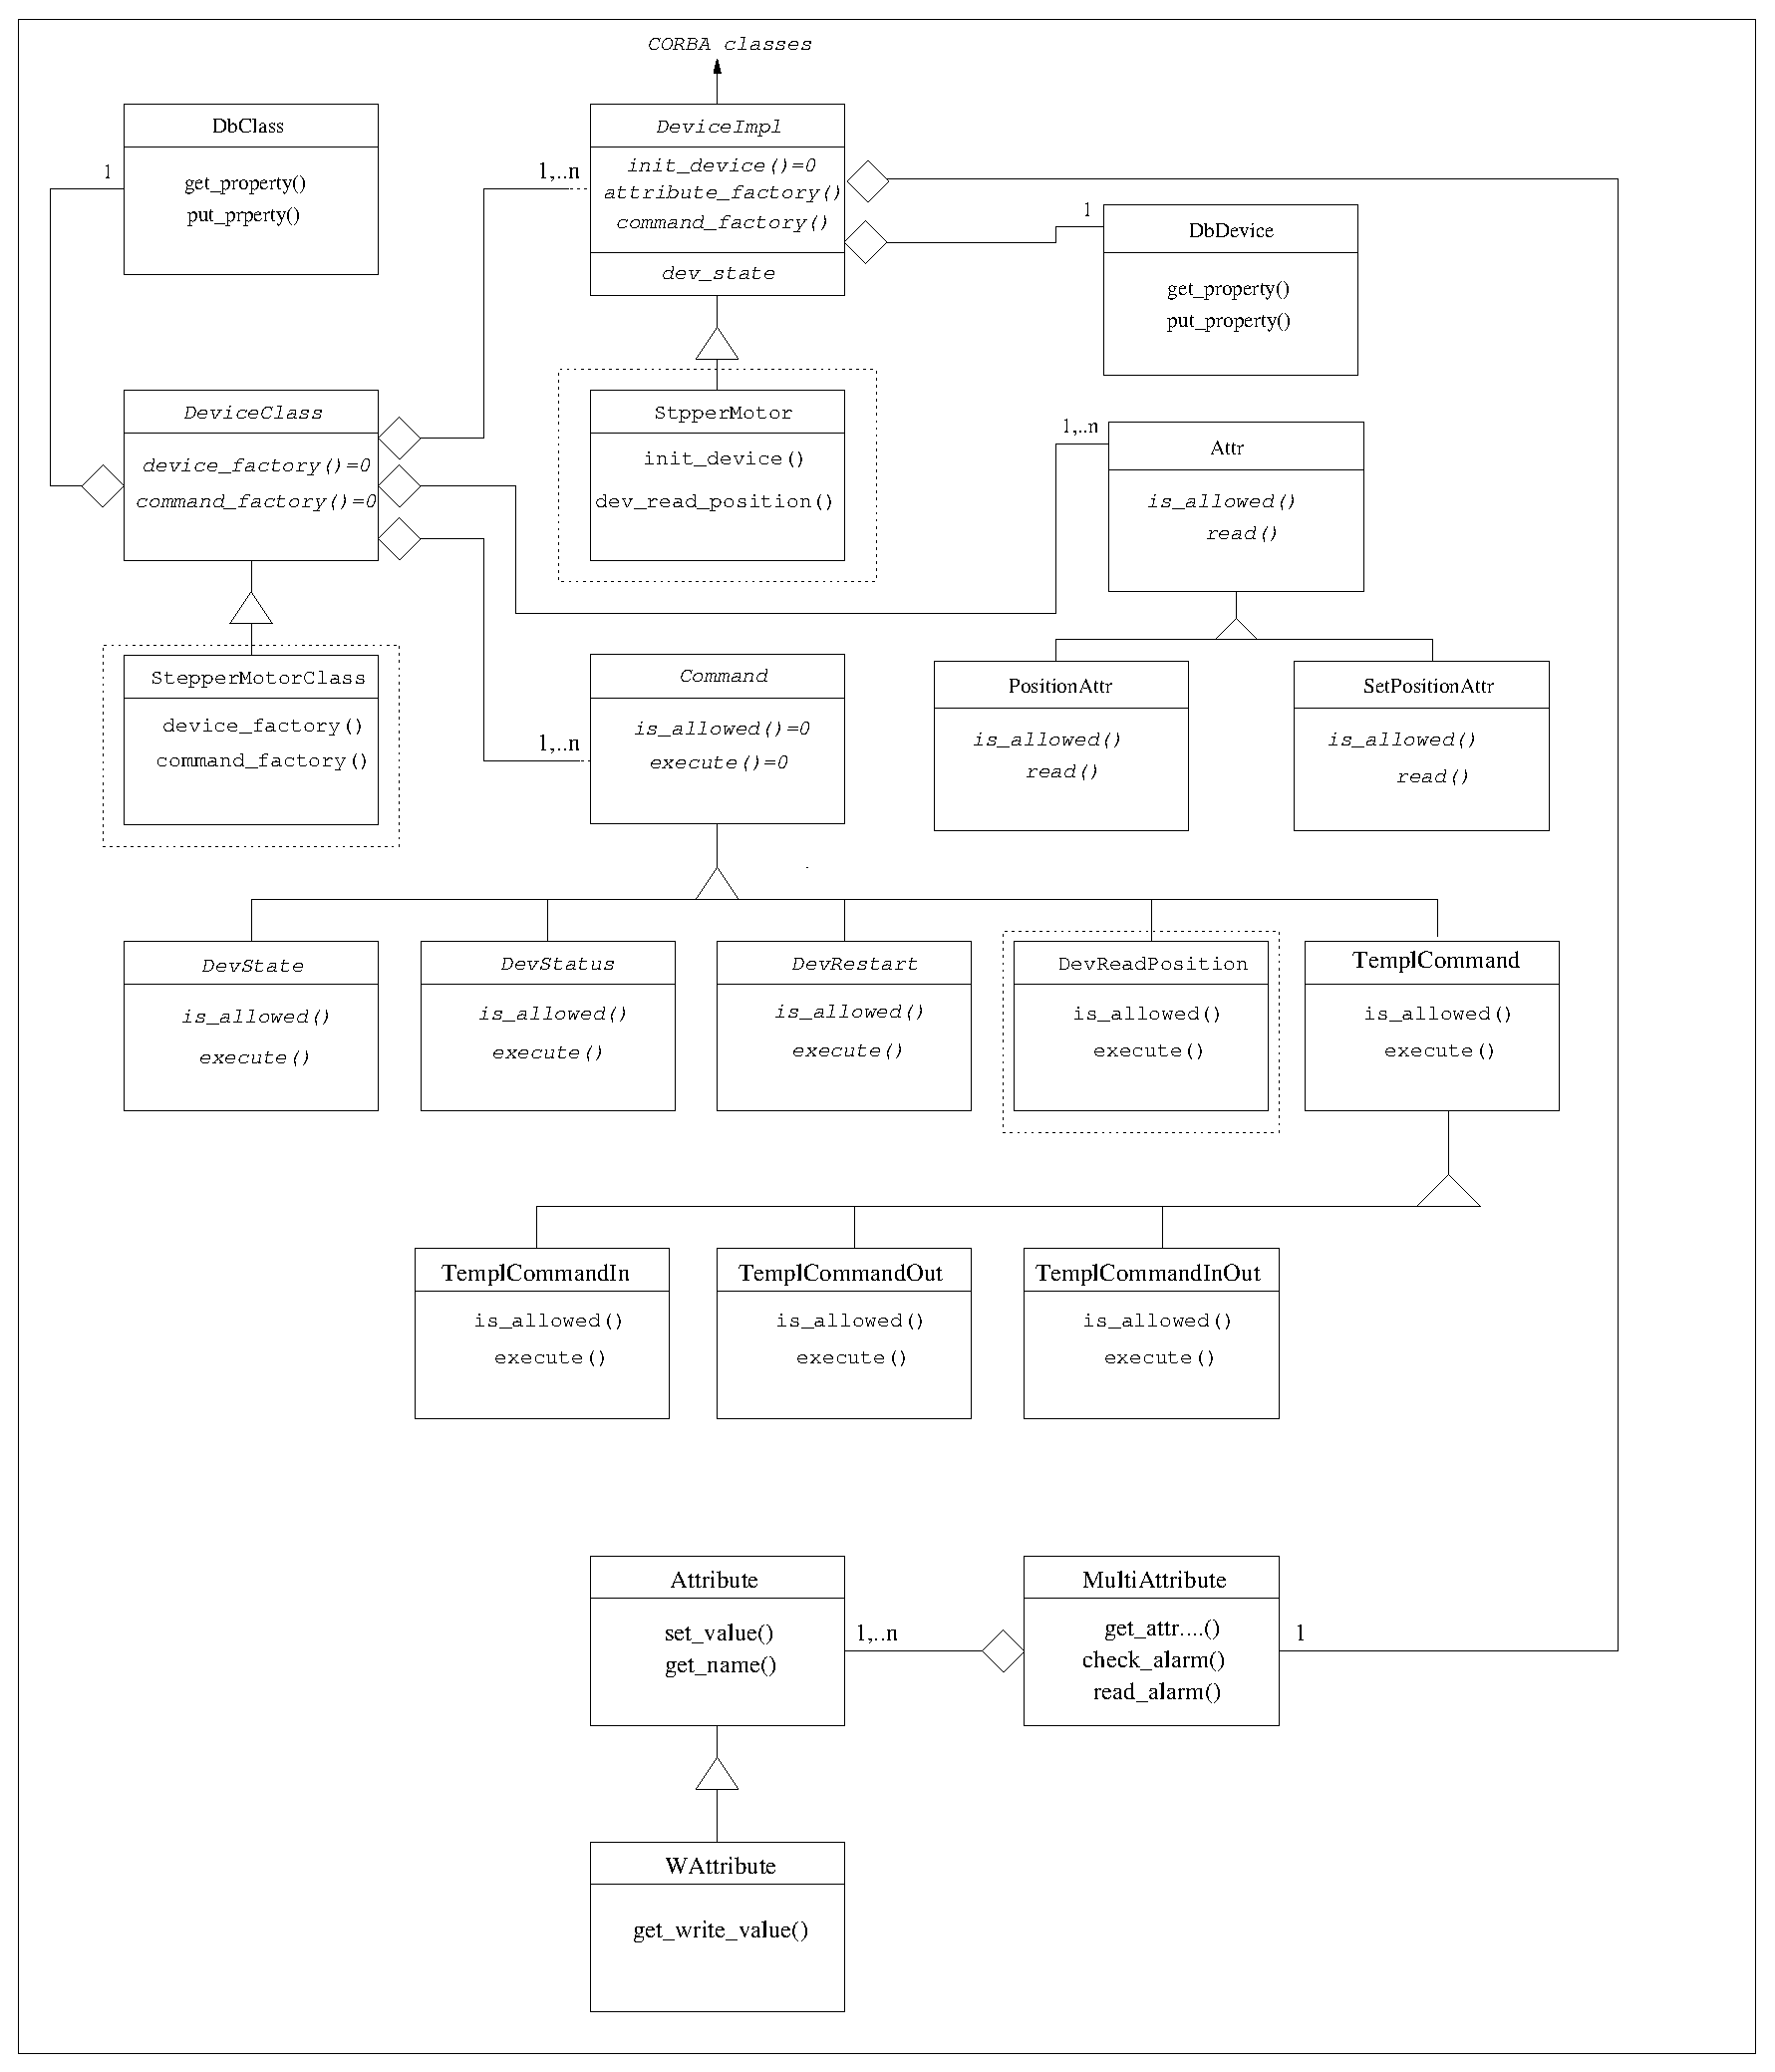
\includegraphics[width=14cm,height=18cm]{ds_writing/device_et}}
\par\end{centering}

\protect\caption{Device pattern class diagram}
\label{Dvice pattern figure}
\end{figure}
. In this figure, only classes surrounded with a dash line square
are device specific. All the other classes are part of the TDSOM core
and are developed by the Tango system team. Different kind of classes
are used by the device pattern. 
\begin{itemize}
\item Three of them are root classes and it is only necessary to inherit
from them. These classes are the \textbf{DeviceImpl}\index{DeviceImpl},
\textbf{DeviceClass\index{DeviceClass}} and \textbf{Command\index{Command}}
classes. 
\item Classes necessary to implement commands\index{command}. The TDSOM
supports two ways to create command : Using inheritance\index{inheritance}
or using the template\index{template} command model. It is possible
to mix model within the same device pattern

\begin{enumerate}
\item Using \textbf{inheritance}. This model of creating command heavily
used the polymorphism offered by each modern object oriented programming
language. In this schema, each command supported by a device via the
command\_inout\index{command-inout} or command\_inout\_async\index{command-inout-async}
operation is implemented by a separate class. The Command\index{Command}
class is the root class for each of these classes. It is an abstract
class. A \emph{execute\index{execute}} method must be defined in
each sub-class. A \emph{is\_allowed\index{is-allowed}} method may
also be re-defined in each class if the default one does not fulfill
all the needs%
\footnote{The default is\_allowed method behavior is to always allows the command%
}. In our stepper motor device server example, the DevReadPosition
command follows this model.
\item Using the \textbf{template command} model. Using this model, it is
not necessary to write one class for each command. You create one
instance of classes already defined in the TDSOM for each command.
The link between command name and method which need to be executed
is done through pointers to method. To support different kind of command,
four classes are part of the TDSOM. These classes are :

\begin{enumerate}
\item The \textbf{TemplCommand\index{TemplCommand}} class for command without
input or output parameter
\item The \textbf{TemplCommandIn\index{TemplCommandIn}} class for command
with input parameter but without output parameter
\item The \textbf{TemplCommandOu}t\index{TemplCommandOut} class for command
with output parameter but without input parameter
\item The \textbf{TemplCommandInOut\index{TemplCommandInOut}} class for
all the remaining commands
\end{enumerate}
\end{enumerate}
\item Classes necessary to implement TANGO device attributes\index{attribute}.
All these classes are part of the TANGO core classes. These classes
are the \textbf{MultiAttribute}\index{MultiAttribute}, \textbf{Attribute\index{Attribute}},
\textbf{WAttribute\index{WAttribute}}, \textbf{Attr}\index{Attr},
\textbf{SpectrumAttr\index{SpectrumAttr}} and \textbf{ImageAttr\index{ImageAttr}}
classes. The last three are used to create user attribute. Each attribute
supported by a device is implemented by a separate class. The Attr
class is the root class for each of these classes. According to the
attribute data format, the user class implementing the attribute must
inherit from the Attr, SpectrumAttr or ImageAtttr class. SpectrumAttr
class inherits from Attr class and Image Attr class inherits from
the SpectrumAttr class. The Attr base class defined three methods
called \emph{is\_allowed}\index{is-allowed}, \emph{read\index{read}}
and \emph{write}\index{write}. These methods may be redefined in
sub-classes in order to implement the attribute specific behaviour.
\item The other are device specific. For stepper motor device, they are
named StepperMotor, StepperMotorClass and DevReadPosition.
\end{itemize}

\subsubsection{The Tango base class (DeviceImpl\index{DeviceImpl} class)}


\paragraph{Description}

This class is the device root class and is the link between the Device
pattern\index{pattern} and CORBA\index{CORBA}. It inherits from
CORBA classes and implements all the methods needed to execute CORBA
operations and attributes. For instance, its method \emph{command\_inout\index{command-inout}}
is executed when a client requests a command\_inout operation. The
method \emph{name\index{name}} of the DeviceImpl class is executed
when a client requests the name CORBA attribute. This class also encapsulates
some key device data like its name\index{name}, its state\index{state},
its status\index{status}, its black box\index{black-box}.... This
class is an abstract class and cannot be instantiated as is. 


\paragraph{Contents}

The contents of this class can be summarized as :
\begin{itemize}
\item Different constructors and one destructor
\item Methods to access instance data members outside the class or its derivate
classes. These methods are necessary because data members are declared
as protected.
\item Methods triggered by CORBA attribute request
\item Methods triggered by CORBA operation\index{operation} request
\item The \emph{init\_device\index{init-device}()} method. This method
makes the class abstract. It should be implemented by a sub-class.
It is used by the inherited classes constructors.
\item Methods triggered by the automatically added State\index{State} and
Status\index{Status} commands. These methods are declared virtual
and therefore can be redefined in sub-classes. These two commands
are automatically added to the list of commands defined for a class
of devices. They are discussed in chapter \ref{Auto_cmd}
\item A method called \emph{always\_executed\_hook()\index{always-executed-hook}}
always executed for each command before the device state is tested
for command execution. This method gives the programmer a hook where
he(she) can program some mandatory action which must be done before
any command execution. An example of the such action is an hardware
access to the device to read its real hardware state.
\item A method called \emph{read\_attr\_hardware()}\index{read-attr-hardware}
triggered by the read\_attributes\index{read-attributes} CORBA operation.
This method is called once for each read\_attributes\index{read-attributes}
call. This method is virtual and may be redefined in sub-classes. 
\item A method called \emph{write\_attr\_hardware()}\index{write-attr-hardware}
triggered by the write\_attributes\index{write-attributes} CORBA
operation. This method is called once for each write\_attributes\index{write-attributes}
call. This method is virtual and may be redefined in sub-classes. 
\item Methods for signal\index{signal} management (C++ specific) 
\item Data members like the device name\index{name}, the device status\index{status},
the device state\index{state}
\item Some private methods and data members
\end{itemize}

\subsubsection{The DbDevice class}

Each DeviceImpl instance is an aggregate with one instance of the
DbDevice\index{DbDevice} class. This DbDevice class can be used to
query or modify device properties\index{properties}. It provides
an easy to use interface for device objects in the database. The description
of this class can be found in the Tango API reference documentation
available on the Tango WEB pages.


\subsubsection{The Command class}


\paragraph{Description of the inheritance\index{inheritance} model}

Within the TDSOM, each command\index{command} supported by a device
and implemented using the inheritance model is implemented by a separate
class. The Command\index{Command} class is the root class for each
of these classes. It is an abstract class. It stores the command name,
the command argument types and description and mainly defines two
methods which are the \emph{execute} and \emph{is\_allowed\index{is-allowed}}
methods. The \emph{execute\index{execute}} method should be implemented
in each sub-class. A default \emph{is\_allowed} method exists for
command always allowed. A command also stores a parameter which is
the command display type. It is also used to select if the command
must be displayed according to the application mode (every day operation
or expert mode).


\paragraph{Description of the template model}

Using this method, it is not necessary to create a separate class
for each device command. In this method, each command is represented
by an instance of one of the template\index{template} command classes.
They are four template command classes. All these classes inherits
from the Command class. These four classes are :
\begin{enumerate}
\item The \textbf{TemplCommand\index{TemplCommand}} class. One object of
this class must be created for each command without input nor output
parameters
\item The \textbf{TemplCommandIn\index{TemplCommandIn}} class. One object
of this class must be created for each command without output parameter
but with input parameter
\item The \textbf{TemplCommandOut\index{TemplCommandOut}} class. One object
of this class must be created for each command without input parameter
but with output parameter
\item The \textbf{TemplCommandInOut\index{TemplCommandInOut}} class. One
object of this class must be created for each command with input and
output parameters
\end{enumerate}
These four classes redefine the \emph{execute\index{execute}} and
\emph{is\_allowed\index{is-allowed}} method of the Command class.
These classes provides constructors which allow the user to :
\begin{itemize}
\item specify which method must be executed by these classes \emph{execute}
method
\item optionally specify which method must be executed by these classes
\emph{is\_allowed} method.
\end{itemize}
The method specification is done via pointer to method.

Remember that it is possible to mix command implementation method
within the same device pattern.


\paragraph{Contents}

The content of this class can be summarizes as :
\begin{itemize}
\item Class constructors and destructor
\item Declaration of the \emph{execute\index{execute}} method
\item Declaration of the \emph{is\_allowed\index{is-allowed}} method
\item Methods to read/set class data members
\item Methods to extract\index{extract} data from the object used to transfer
data on the network
\item Methods to insert\index{insert} data into the object used to transfer
data on the network
\item Class data members like command name, command input data type, command
input data description...
\end{itemize}

\subsubsection{The DeviceClass\index{DeviceClass} class}


\paragraph{Description}

This class implements all what is specific for a controlled object
class. For instance, every device of the same class supports the same
list of commands\index{command} and therefore, this list of available
commands is stored in this DeviceClass. The structure returned by
the info operation contains a documentation URL%
\footnote{URL stands for \textbf{U}niform \textbf{R}esource \textbf{L}ocator%
}. This documentation\index{documentation} URL\index{URL} is the
same for every device of the same class. Therefore, the documentation
URL is a data member of this class. There should have only one instance
of this class per device pattern implementation. The device list is
also stored in this class. It is an abstract class because the two
methods \emph{device\_factory\index{device-factory}()} and \emph{command\_factory\index{command-factory}()}
are declared as pure virtual. The rule of the \emph{device\_factory()}
method is to create all the devices belonging to the device class.
The rule of the \emph{command\_factory()} method is to create one
instance of all the classes needed to support device commands. This
class also stored the \emph{attribute\_factory\index{attribute-factory}}
method. The rule of this method is to store in a vector of strings,
the name of all the device attributes. This method has a default implementation
which is an empty body for device without attribute\index{attribute}.


\paragraph{Contents}

The contents of this class can be summarize as :
\begin{itemize}
\item The \emph{command\_handler\index{command-handler}} method
\item Methods to access data members.
\item Signal\index{signal} related method (C++ specific)
\item Class constructor. It is protected to implements the Singleton pattern
\item Class data members like the class command list, the device list...
\end{itemize}

\subsubsection{The DbClass\index{DbClass} class}

Each DeviceClass instance is an aggregate with one instance of the
DbClass class. This DbClass class can be used to query or modify class
properties\index{properties}. It provides an easy to use interface
for device objects in the database. The description of this class
can be found in the reference Tango C++ API documentation available
in the Tango WEB pages.


\subsubsection{The MultiAttribute\index{MultiAttribute} class}


\paragraph{Description}

This class is a container for all the TANGO attributes defined for
the device. There is one instance of this class for each device. This
class is mainly an aggregate of Attribute object(s). It has been developed
to ease TANGO attribute management.


\paragraph{Contents}

The class contents could be summarizes as :
\begin{itemize}
\item Miscellaneous methods to retrieve one attribute\index{attribute}
object in the aggregate
\item Method to retrieve a list of attribute with an alarm level defined
\item Get attribute number method
\item Miscellaneous methods to check if an attribute value is outside the
authorized limits
\item Method to add messages for all attribute with an alarm set
\item Data members with the attribute list
\end{itemize}

\subsubsection{The Attribute\index{Attribute} class}


\paragraph{Description}

There is one object of this class for each device attribute\index{attribute}.
This class is used to store all the attribute properties\index{properties},
the attribute value and all the alarm\index{alarm} related data.
Like commands, this class also stores th attribute display type. It
is foreseen to be used by future Tango graphical application toolkit
to select if the attribute must be displayed according to the application
mode (every day operation or expert mode).


\paragraph{Contents}
\begin{itemize}
\item Miscellaneous method to get boolean attribute information
\item Methods to access some data members
\item Methods to get/set attribute properties
\item Method to check if the attribute is in alarm condition
\item Methods related to attribute data
\item Friend function to print attribute properties
\item Data members (properties value and attribute data)
\end{itemize}

\subsubsection{The WAttribute\index{WAttribute} class}


\paragraph{Description}

This class inherits from the Attribute class. There is one instance
of this class for each writable\index{writable} device attribute.
On top of all the data already managed by the Attribute class, this
class stores the attribute set value.


\paragraph{Contents}

Within this class, you will mainly find methods related to attribute\index{attribute}
set value storage and some data members.


\subsubsection{The Attr class}

Within the TDSOM, each attribute\index{command} supported by a device
is implemented by a separate class. The Attr\index{Attr} class is
the root class for each of these classes. It is used in conjonction
with the Attribute and Wattribute classes to implement Tango attribute
behaviour. It defines three methods which are the \emph{is\_allowed\index{is-allowed},
read} and \emph{write} methods. A default \emph{is\_allowed} method
exists for attribute always allowed. Default \emph{read} and \emph{write}
empty methods are defined. For readable attribute, it is necessary
to overwrite the \emph{read} method. For writable attribute, it is
necessary to overwrite the \emph{write} method and for read and write
attribute, both methods must be overwritten.


\subsubsection{The SpectrumAttr\index{SpectrumAttr} class}

This class inherits from the Attr class. It is the base class for
user spectrum attribute. It is used in conjonction with the Attribute
and WAttribute class to implement Tango spectrum attribute behaviour.
From the Attr class, it inherits the Attr \emph{is\_allowed}, \emph{read}
and \emph{write} methods.


\subsubsection{The ImageAttr\index{ImageAttr} class}

This class inherits from the SpectrumAttr class. It is the base class
for user image attribute. It is used in conjonction with the Attribute
and WAttribute class to implement Tango image attribute behaviour.
From the Attr class, it inherits the Attr \emph{is\_allowed}, \emph{read}
and \emph{write} methods.


\subsubsection{The StepperMotor class}


\paragraph{Description}

This class inherits from the DeviceImpl\index{DeviceImpl} class and
is the class implementing the controlled object behavior. Each command
will trigger a method in this class written by the device server programmer
and specific to the object to be controlled. This class also stores
all the device specific data.


\paragraph{Definition}


\begin{minted}[linenos]{cpp}
1 class StepperMotor: public TANGO_BASE_CLASS
2 {
3 public :
4    StepperMotor(Tango::DeviceClass *,string &);
5    StepperMotor(Tango::DeviceClass *,const char *);
6    StepperMotor(Tango::DeviceClass *,const char *,const char *);
7    ~StepperMotor() {};
8 
9    DevLong dev_read_position(DevLong);
10   DevLong dev_read_direction(DevLong);
11   bool direct_cmd_allowed(const CORBA::Any &);
12 
13   virtual Tango::DevState dev_state();
14   virtual Tango::ConstDevString dev_status();
15 
16   virtual void always_executed_hook();
17 
18   virtual void read_attr_hardware(vector<long> &attr_list);
19   virtual void write_attr_hardware(vector<long> &attr_list);
20 
21   void read_position(Tango::Attribute &);
22   bool is_Position_allowed(Tango::AttReqType req);
23   void write_SetPosition(Tango::WAttribute &);
24   void read_Direction(Tango::Attribute &);
25 
26   virtual void init_device();
27   virtual void delete_device();
28 
29   void get_device_properties();
30 
31 protected : 
32   long axis[AGSM_MAX_MOTORS];
33   DevLong position[AGSM_MAX_MOTORS];
34   DevLong direction[AGSM_MAX_MOTORS];
35   long state[AGSM_MAX_MOTORS];
36 
37   Tango::DevLong *attr_Position_read;
38   Tango::DevLong *attr_Direction_read;
38   Tango::DevLong attr_SetPosition_write;
40 
41   Tango::DevLong min;
42   Tango::DevLong max;
43 
44   Tango::DevLong *ptr;
45 };
46 
47 } /* End of StepperMotor namespace */
\end{minted}


Line 1 : The StepperMotor class inherits from the DeviceImpl class

Line 4-7 : Class constructors and destructor

Line 9 : Method triggered by the DevReadPosition command

Line 10-11 : Methods triggered by the DevReadDirection command

Line 13 : Redefinition of the \emph{dev\_state\index{dev-state}}
method of the DeviceImpl class. This method will be triggered by the
State\index{State} command

Line 14 : Redefinition of the \emph{dev\_statu}\index{dev-status}s
method of the DeviceImpl class. This method will be triggered by the
Status\index{Status} command

Line 16 : Redefinition of the \emph{always\_executed\_hook\index{always-executed-hook}}
method.

Line 26 : Definition of the \emph{init\_device\index{init-device}}
method (declared as pure virtual by the DeviceImpl class)

Line 27 : Definition of the \emph{delete\_device}\index{delet-device}
method

Line 31-45 : Device data


\subsubsection{The StepperMotorClass class}


\paragraph{Description}

This class inherits from the DeviceClass\index{DeviceClass} class.
Like the DeviceClass class, there should be only one instance of the
StepperMotorClass. This is ensured because this class is written following
the Singleton\index{singleton} pattern as defined in \cite{Patterns}.
All controlled object class data which should be defined only once
per class must be stored in this object.


\paragraph{Definition }



     1  class StepperMotorClass : public DeviceClass

     2  \{

3  public:

     4          static StepperMotorClass {*}init(const char {*});

     5          static StepperMotorClass {*}instance();

     6          \textasciitilde{}StepperMotorClass() \{\_instance
= NULL;\}

     7          

     8  protected:

     9          StepperMotorClass(string \&);

    10          static StepperMotorClass {*}\_instance;

    11          void command\_factory();

    12          

    13  private:

    14          void device\_factory(Tango\_DevVarStringArray {*});

    15  \};



Line 1 : This class is a sub-class of the DeviceClass class

Line 4-5 and 9-10: Methods and data member necessary for the Singleton\index{singleton}
pattern

Line 6 : Class destructor

Line 11 : Definition of the \emph{command\_factor\index{command-factory}y}
method declared as pure virtual in the DeviceClass call

Line 13-14 : Definition of the \emph{device\_factory\index{device-factory}}
method declared as pure virtual in the DeviceClass class


\subsubsection{The DevReadPosition class}


\paragraph{Description}

This is the class for the DevReadPosition command. This class implements
the \emph{execute\index{execute}} and \emph{is\_allowed\index{is-allowed}}
methods defined by the Command\index{Command} class. This class is
necessary because this command is implemented using the inheritance\index{inheritance}
model.


\paragraph{Definition}


\begin{minted}[linenos]{cpp}
1  class DevReadPositionCmd : public Command
2  {
3  public:
4      DevReadPositionCmd(const char *,Tango_CmdArgType, Tango_CmdArgType, const char *, const char*);
5      ~DevReadPositionCmd() {};
6          
7      virtual bool is_allowed (DeviceImpl *, const CORBA::Any &);
8      virtual CORBA::Any *execute (DeviceImpl *, const CORBA::Any &);
9  };
\end{minted}


Line 1 : The class is a sub class of the Command class

Line 4-5 : Class constructor and destructor

Line 7-8 : Definition of the \emph{is\_allowed} and \emph{execute}
method declared as pure virtual in the Command class.


\subsubsection{The PositionAttr class}


\paragraph{Description}

This is the class for the Position attribute. This attribute is a
scalar attribute and therefore inherits from the Attr base class.
This class implements the \emph{read\index{execute}} and \emph{is\_allowed\index{is-allowed}}
methods defined by the Attr\index{Command} class.


\paragraph{Definition}


\begin{minted}[linenos]{cpp}
     1  class PositionAttr: public Tango::Attr
     2  {
     3  public:
     4     PositionAttr():Attr("Position",Tango::DEV_LONG,Tango::READ);
     5     ~PositionAttr() {};
     6          
     7     virtual void read(Tango::DeviceImpl *dev,Tango::Attribute &att)
     8     {(static_cast<StepperMotor *>(dev))->read_Position(att);}
     9     virtual bool is_allowed(Tango::DeviceImpl *dev,Tango::AttReqType ty)
    10     {return (static_cast<StepperMotor *>(dev))->is_Position_allowed(ty);}
    11  };
\end{minted}


Line 1 : The class is a sub class of the Attr class

Line 4-5 : Class constructor and destructor

Line 7 : Re-definition of the \emph{read} method defined in the Attr
class. This is simply a \textquotedbl{}forward\textquotedbl{} to the
\emph{read\_Position} method of the StepperMotor class

Line 9 : Re-definition of the \emph{is\_allowed} method defined in
the Attr class. This is also a \textquotedbl{}forward\textquotedbl{}
to the \emph{is\_Position\_allowed} method of the StepperMotor class


\subsection{Startup of a device pattern}
\label{Pattern startup}

To start the device pattern implementation for stepper motor device,
four methods of the StepperMotorClass class must be executed. These
methods are :
\begin{enumerate}
\item The creation of the StepperMethodClass singleton\index{singleton}
via its \emph{init}() method
\item The \emph{command\_factory}()\index{command-factory} method of the
StepperMotorClass class
\item The \emph{attribute\_factory}\index{attribute-factory}() method of
the StepperMotorClass class. This method has a default empty body
for device class without attributes.
\item The \emph{device\_factory}\index{device-factory}() method of the
StepperMotorClass class
\end{enumerate}
This startup procedure is described in figure \ref{pattern_startup_fig}
\begin{figure}
\begin{centering}
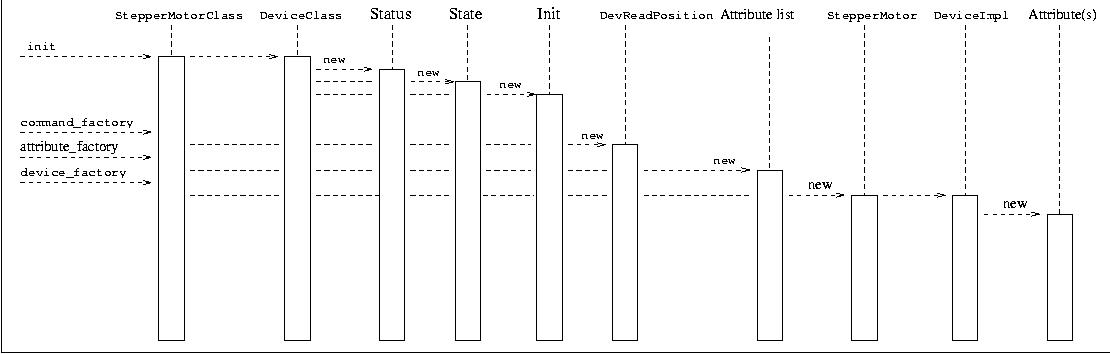
\includegraphics[width=14cm,height=10cm]{ds_writing/startup}
\par\end{centering}

\protect\caption{Device pattern startup sequence}
\label{pattern_startup_fig}
\end{figure}
 . The creation of the StepperMotorClass will automatically create
an instance of the DeviceClass class. The constructor of the DeviceClass\index{DeviceClass}
class will create the Status\index{Status}, State\index{State} and
Init\index{Init} command objects and store them in its command list.

The \emph{command\_factory}() method will simply create all the user
defined commands and add them in the command list.

The \emph{attribute\_factory}() method will simply build a list of
device attribute names.

The \emph{device\_factory}() method will create each StepperMotor
object and store them in the StepperMotorClass instance device list.
The list of devices to be created and their names is passed to the
\emph{device\_factory} method in its input argument. StepperMotor
is a sub-class of DeviceImpl class. Therefore, when a StepperMotor
object is created, a DeviceImpl object is also created. The DeviceImpl
constructor builds all the device attribute object(s) from the attribute
list built by the \emph{attribute\_factory()} method.


\subsection{Command execution sequence}

The figure \ref{command_timing_fig}
\begin{figure}[H]
\begin{centering}
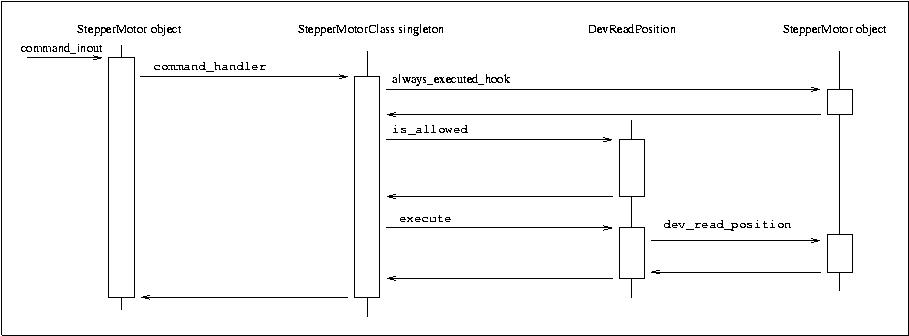
\includegraphics[width=14cm,height=8cm]{ds_writing/command}
\par\end{centering}

\protect\caption{Command execution timing}
\label{command_timing_fig}
\end{figure}
 described how the method implementing a command is executed when
a command\_inout\index{command-inout} CORBA operation is requested
by a client. The \emph{command\_inout} method of the StepperMotor
object (inherited from the DeviceImpl class) is triggered by an instance
of a class generated by the CORBA\index{CORBA} IDL compiler. This
method calls the \emph{command\_handler}()\index{command-handler}
method of the StepperMotorClass object (inherited from the DeviceClass
class). The \emph{command\_handler} method searches in its command\index{command}
list for the wanted command (using its name). If the command is found,
the \emph{always\_executed\_hook\index{always-executed-hook}} method
of the StepperMotor object is called. Then, the \emph{is\_allowed\index{is-allowed}}
method of the wanted command is executed. If the \emph{is\_allowed}
method returns correctly, the \emph{execute\index{execute}} method
is executed. The \emph{execute} method extracts the incoming data
from the CORBA object use to transmit data over the network and calls
the user written method which implements the command.


\subsection{The automatically added commands}
\label{Auto_cmd}

In order to increase the common behavior of every kind of devices
in a TANGO control system, three commands are automatically added
to each class of devices. These commands are :
\begin{itemize}
\item State\index{State}
\item Status\index{Status}
\item Init\index{Init}
\end{itemize}
The default behavior of the method called by the State command depends
on the device state. If the device state is ON or ALARM\index{ALARM},
the method will :
\begin{itemize}
\item read the attribute(s) with an alarm\index{alarm} level defined
\item check if the read value is above/below the alarm level and eventually
change the device state to ALARM.
\item returns the device state.
\end{itemize}
For all the other device state\index{state}, the method simply returns
the device state stored in the DeviceImpl class. Nevertheless, the
method used to return this state (called \emph{dev\_state}\index{state})
is defined as virtual and can be redefined in DeviceImpl sub-class.
The difference between the default State command and the state CORBA
attribute is the ability of the State\index{State} command to signal
an error to the caller by throwing an exception.

The default behavior of the method called by the Status\index{Status}
command depends on the device state. If the device state is ON or
ALARM\index{ALARM}, the method returns the device status stored in
the DeviceImpl class plus additional message(s) for all the attributes
which are in alarm condition. For all the other device state, the
method simply returns the device status as it is stored in the DeviceImpl
class. Nevertheless, the method used to return this status (called
\emph{dev\_status}\index{status}) is defined as virtual and can be
redefined in DeviceImpl sub-class. The difference between the default
Status command and the status CORBA attribute is the ability of the
Status command to signal an error to the caller by throwing an exception.

The Init\index{Init} command is used to re-initialize a device without
changing its network connection. This command calls the device \emph{delete\_device\index{delete-device}}
method and the device \emph{init\_device\index{init-device}} method.
The rule of the \emph{delete\_device} method is to free memory allocated
in the \emph{init\_device} method in order to avoid memory leak.


\subsection{Reading/Writing attributes}


\subsubsection{Reading attributes}

A Tango client is able to read Tango attribute\index{attribute}(s)
with the CORBA read\_attributes\index{read-attributes} call. Inside
the device server, this call will trigger several methods of the device
class (StepperMotor in our example) :
\begin{enumerate}
\item The \emph{always\_executed\_hook()\index{allways-executed-hook}}
method. 
\item A method call \emph{read\_attr\_hardware()}\index{read-attr-hardware}.
This method is called one time per read\_attributes CORBA call. The
aim of this method is to read the device hardware and to store the
result in a device class data member.
\item For each attribute to be read

\begin{enumerate}
\item A method called \emph{is\_<att name>\_allowed()}. The rule of this
method is to allow (or disallow) the next method to be executed. It
is usefull for device with some attributes which can be read only
in some precise conditions. It has one parameter which is the request
type (read or write)
\item A method called \emph{read\_<att name>()}. The aim of this method
is to extract the real attribute value from the hardware read-out
and to store the attribute value into the attribute object. It has
one parameter which is a reference to the Attribute object to be read.
\end{enumerate}
\end{enumerate}
The figure \ref{r_attribute_timing_fig} is a drawing of these method
calls sequencing. For attribute always readable, a default \emph{is\_allowed}
method is provided. This method always returns true.
\begin{figure}[H]
\begin{centering}
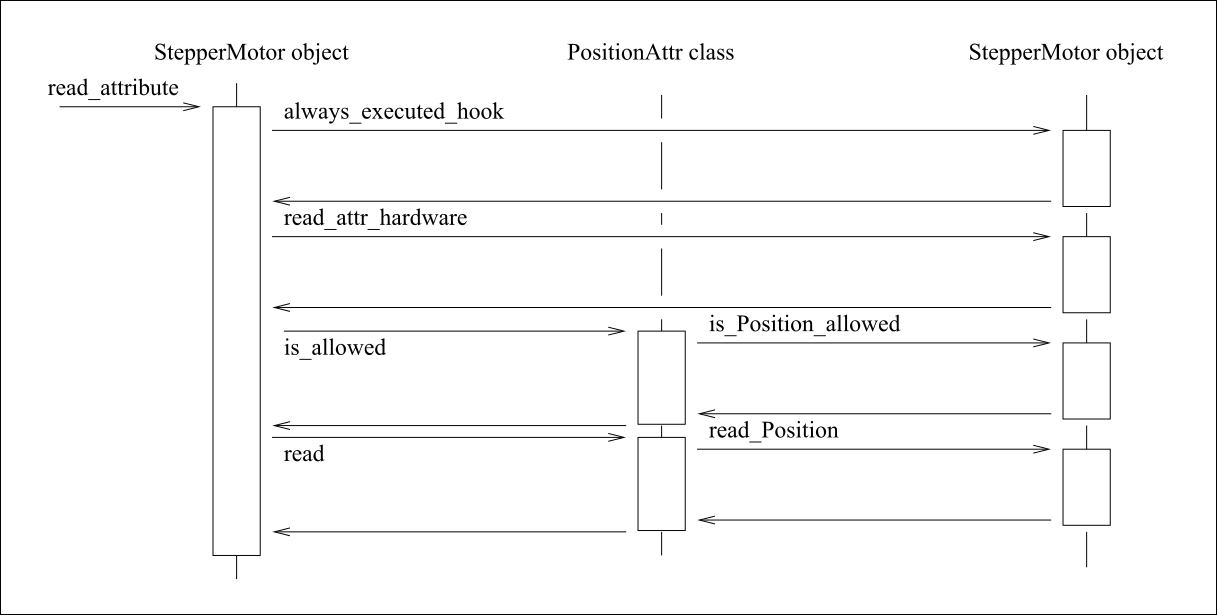
\includegraphics[scale=0.7]{ds_writing/r_attribute}
\par\end{centering}

\protect\caption{Read attribute sequencing}
\label{r_attribute_timing_fig}
\end{figure}



\subsubsection{Writing attributes}

A Tango client is able to write Tango attribute(s) with the CORBA
write\_attributes\index{write-attributes} call. Inside a device server,
this call will trigger several methods of the device class (StepperMotor
in our example)
\begin{enumerate}
\item The \emph{always\_executed\_hook()\index{allways-executed-hook}}
method. 
\item For each attribute to be written

\begin{enumerate}
\item A method called \emph{is\_<att name>\_allowed()}. The rule of this
method is to allow (or disallow) the next method to be executed. It
is usefull for device with some attributes which can be written only
in some precise conditions. It has one parameter which is the request
type (read or write)
\item A method called \emph{write\_<att name>()}. It has one parameter which
is a reference to the WAttribute object to be written. The aim of
this method is to get the data to be written from the WAttribute object
and to write this value into the corresponding hardware. If the hardware
support writing several data in one go, code the hardware access in
the \emph{write\_attr\_harware()} method.
\end{enumerate}
\item The write\_attr\_hardware()\index{write-attr-hardware} method. The
rule of this method is to effectively write the hardware in case it
is able to support writing several data in one go. If this is not
the case, don't code this method (a default implementation is coded
in the Tango base class) and code the real hardware access in each
\emph{write\_<att name>()} method.
\end{enumerate}
The figure \ref{w_attribute_timing_fig} is a drawing of these method
calls sequencing. For attribute always writeable, a default is\_allowed
method is provided. This method always allways returns true.
\begin{figure}[H]
\begin{centering}
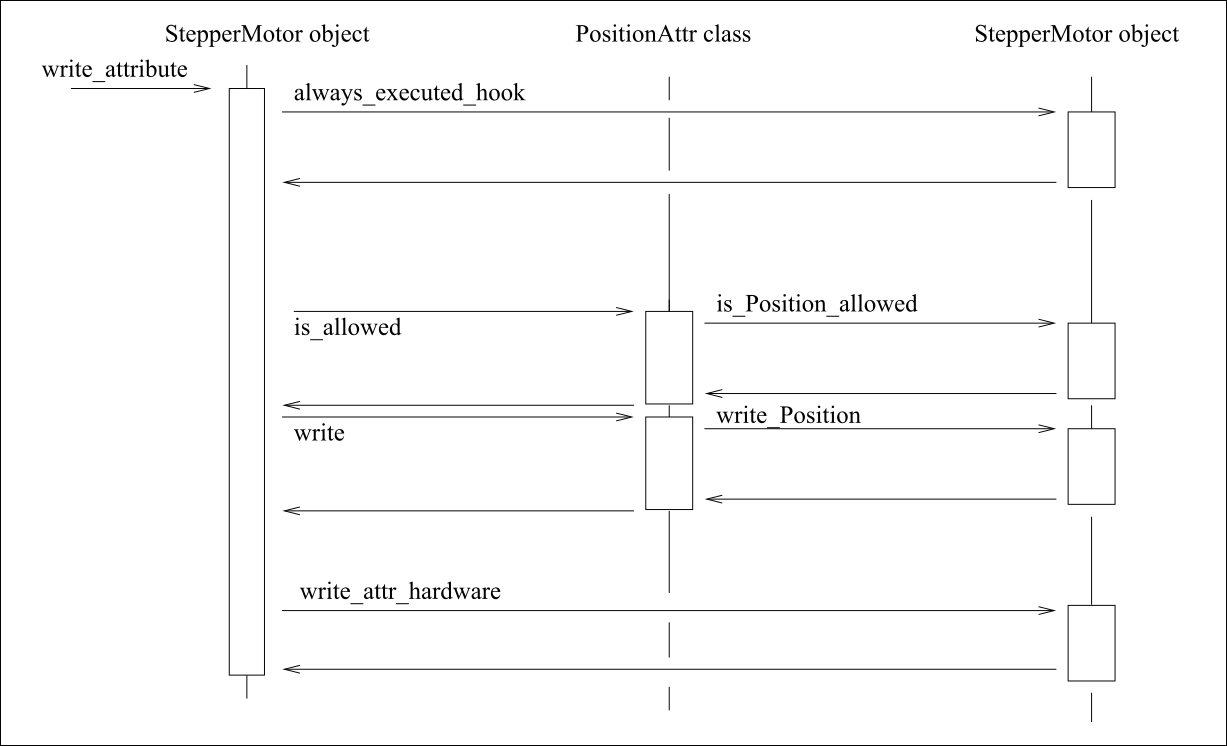
\includegraphics[scale=0.7]{ds_writing/w_attribute}
\par\end{centering}

\protect\caption{Write attribute sequencing}
\label{w_attribute_timing_fig}
\end{figure}



\subsection{The device server framework}


\subsubsection{Vocabulary}
\label{Voc}

A device server\index{server} pattern implementation is embedded
in a process called a \textbf{device server}. Several instances of
the same device server process can be used in a TANGO control system.
To identify instances, a device server process is started with an
\textbf{instance name} which is different for each instance. The device
server name is the couple device server executable\index{executable}
name/device server instance\index{instance} name. For instance, a
device server started with the following command \begin{center}Perkin
id11\end{center} starts a device server process with an instance
name id11, an executable name Perkin and a device server name Perkin/id11.


\subsubsection{The DServer class}
\label{DServer_class}

In order to simplify device server process administration, a device
of the DServer\index{DServer} class is automatically added to each
device server process. Thus, every device server process supports
the same set of administration\index{administration} commands. The
implementation of this DServer class follows the device pattern and
therefore, its device behaves like any other devices. The device name
is \begin{center}dserver/device server executable name/device server
instance name\end{center}For instance, for the device server process
described in chapter \ref{Voc}, the dserver device name is dserver/perkin/id11.
This name is returned by the adm\_name\index{adm-name} CORBA attribute
available for every device. On top of the three automatically added
commands, this device supports the following commands :
\begin{itemize}
\item DevRestart\index{DevRestart}
\item RestartServer\index{RestartServer}
\item QueryClass\index{QueryClass}
\item QueryDevice\index{QueryDevice}
\item Kill\index{Kill}
\item AddLoggingTarget (C++ server only)\index{AddLoggingTarget}
\item RemoveLoggingTarget (C++ server only)\index{RemoveLoggingTarget}
\item GetLoggingTarget (C++ server only)\index{GetLoggingTarget}
\item GetLoggingLevel (C++ server only)\index{GetLoggingLevel}
\item SetLoggingLevel (C++ server only)\index{SetLoggingLevel}
\item StopLogging (C++ server only)\index{StopLogging}
\item StartLogging (C++ server only)\index{StartLogging}
\item PolledDevice\index{PolledDevice}
\item DevPollStatus\index{DevPollStatus}
\item AddObjPolling\index{AddObjPolling}
\item RemObjPolling\index{RemObjPolling}
\item UpdObjPollingPeriod\index{UpdObjPollingPeriod}
\item StartPolling\index{StartPolling}
\item StopPolling\index{StopPolling}
\item EventSubscriptionChange\index{EventSubscriptionChange}
\item ZmqEventSubscriptionChange\index{ZmqEventSubscriptionChange}
\item LockDevice\index{LockDevice}
\item UnLockDevice\index{UnLockDevice}
\item ReLockDevices\index{ReLockDevices}
\item DevLockStatus\index{DevLockStatus}
\end{itemize}
These commands will be fully described later in this document.

Several controlled object classes can be embedded within the same
device server process and it is the rule of this device to create
all these device server patterns and to call their command and device
factories as described in \ref{Pattern startup}. The name and number
of all the classes to be created is known to this device after the
execution of a method called \emph{class\_factory}\index{class-factory}.
It is the user responsibility to write this method.


\subsubsection{The Tango::Util\index{Util} class}


\paragraph{Description}

This class merges a complete set of utilities in the same class. It
is implemented as a singleton\index{singleton} and there is only
one instance of this class per device server process. It is mandatory
to create this instance in order to run a device server. The description
of all the methods implemented in this class can be found in \cite{TANGO_ref_man}.


\paragraph{Contents}

Within this class, you can find :
\begin{itemize}
\item Static method to create/retrieve the singleton object
\item Miscellaneous utility methods like getting the server output trace
level, getting the CORBA\index{CORBA} ORB pointer, retrieving device
server instance name, getting the server PID and more. Please, refer
to \cite{TANGO_ref_man} to get a complete list of all these utility
methods.
\item Method to create the device pattern implementing the DServer class
(\emph{server\_init()}\index{server-init})
\item Method to start the server (\emph{server\_run()}\index{server-run})
\item TANGO database related methods
\end{itemize}

\subsubsection{A complete device server}

Within a complete device server, at least two implementations of the
device server pattern are created (one for the dserver object and
the other for the class of devices to control). On top of that, one
instance of the Tango::Util\index{Util} class must also be created.
\begin{figure}
\begin{centering}
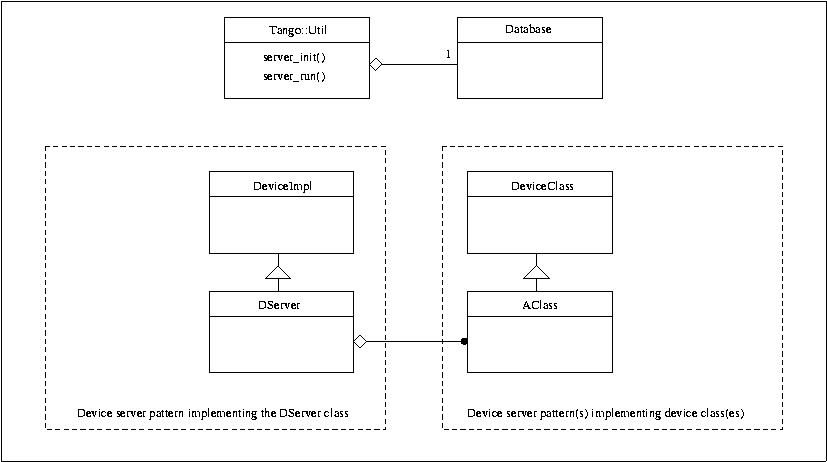
\includegraphics[width=14cm,height=10cm]{ds_writing/complete_server}
\par\end{centering}

\protect\caption{A complete device server}
\label{completeDS}
\end{figure}
 A drawing of a complete device server is in figure \ref{completeDS}


\subsubsection{Device server startup sequence}
\label{Server_startup}

The device server startup sequence is the following :
\begin{enumerate}
\item Create an instance of the Tango::Util class. This will initialize
the CORBA Object Request Broker
\item Called the \emph{server\_init\index{init}} method of the Tango::Util
instance The call to this method will :

\begin{enumerate}
\item Create the DServerClass object of the device pattern implementing
the DServer\index{DServer} class. This will create the dserver object
which during its construction will :

\begin{enumerate}
\item Called the \emph{class\_factory\index{class-factory}} method of the
DServer object. This method must create all the xxxClass instance
for all the device pattern implementation embedded in the device server
process.
\item Call the \emph{command\_factory\index{command-factory}} and \emph{device\_factory\index{device-factory}}
of all the classes previously created. The list of devices passed
to each call to the \emph{device\_factory} method is retrieved from
the TANGO database.
\end{enumerate}
\end{enumerate}
\item Wait for incoming request with the \emph{server\_run()\index{server-run}}
method of the Tango::Util class.
\end{enumerate}

\section{Exchanging data between client and server}
\label{Data exchange}

Exchanging data between clients and server means most of the time
passing data between processes running on different computer using
the network. Tango limits the type of data exchanged between client
and server and defines a way to exchange these data. This chapter
details these features. Memory allocation and error reporting are
also discussed.

\textbf{All the rules described in this chapter are valid only for
data exchanged between client and server. For device server internal
data, classical C++ types can be used.}


\subsection{Command / Attribute data types}

Commands have a fixed calling syntax - consisting of one input argument
and one output argument. Arguments type must be chosen out of a fixed
set of 24 data types. Attributes support a sub-set of these data types
(those are the data type with the (1) note) plus the DevEnum data
type. The following table details type name, code and the corresponding
CORBA IDL types.

The type name used in the type name column of this table is the C++
name. In the IDL file, all the Tango definition are grouped in a IDL\index{IDL}
module named Tango. The IDL module maps to C++ namespace\index{namespace}.
Therefore, all the data type are parts of a namespace called Tango.

\vspace{0.3cm}


\begin{center}
\begin{longtable}{|c|l|}
\hline 
Type name & IDL type\tabularnewline
\hline 
\hline 
Tango::DevBoolean (1) & boolean\tabularnewline
\hline 
Tango::DevShort (1) & short\tabularnewline
\hline 
Tango::DevEnum (2) & short (See chapter on advanced features)\tabularnewline
\hline 
Tango::DevLong (1) & long\tabularnewline
\hline 
Tango::DevLong64 (1) & long long\tabularnewline
\hline 
Tango::DevFloat (1) & float\tabularnewline
\hline 
Tango::DevDouble (1) & double\tabularnewline
\hline 
Tango::DevUShort (1) & unsigned short\tabularnewline
\hline 
Tango::DevULong (1) & unsigned long\tabularnewline
\hline 
Tango::DevULong64 (1) & unsigned long long\tabularnewline
\hline 
Tango::DevString (1) & string\tabularnewline
\hline 
Tango::DevVarCharArray & sequence of unsigned char\tabularnewline
\hline 
Tango::DevVarShortArray & sequence of short\tabularnewline
\hline 
Tango::DevVarLongArray & sequence of long\tabularnewline
\hline 
Tango::DevVarLong64Array & sequence of long long\tabularnewline
\hline 
Tango::DevVarFloatArray & sequence of float\tabularnewline
\hline 
Tango::DevVarDoubleArray & sequence of double\tabularnewline
\hline 
Tango::DevVarUShortArray & sequence of unsigned short\tabularnewline
\hline 
Tango::DevVarULongArray & sequence of unsigned long\tabularnewline
\hline 
Tango::DevVarULong64Array & sequence of unsigned long long\tabularnewline
\hline 
Tango::DevVarStringArray & sequence of string\tabularnewline
\hline 
Tango::DevVarLongStringArray & structure with a sequence of long and a sequence of string\tabularnewline
\hline 
Tango::DevVarDoubleStringArray & structure with a sequence of double and a sequence of string\tabularnewline
\hline 
Tango::DevState (1) & enumeration\tabularnewline
\hline 
Tango::DevEncoded (1) & structure with a string and a sequence of char\tabularnewline
\hline 
\end{longtable}
\par\end{center}

\vspace{0.3cm}


The CORBA Interface Definition Language uses a type called \textbf{sequence}
for variable length array. The Tango::DevUxxx types are used for unsigned
types. The Tango::DevVarxxxxArray must be used when the data to be
transferred are variable length array. The Tango::DevVarLongStringArray\index{Tango::DevVarLongStringArray}
and Tango::DevVarDoubleStringArray\index{Tango::DevVarDoubleStringArray}
are structures with two fields which are variable length array of
Tango long (32 bits) and variable length array of strings for the
Tango::DevVarLongStringArray and variable length array of double and
variable length array of string for the Tango::DevVarDoubleStringArray.
The Tango::State\index{Tango::DevState} type is used by the State\index{State}
command to return the device state. 


\subsubsection{Using data types with C++}

Unfortunately, the mapping between IDL and C++ was defined before
the C++ class library had been standardized. This explains why the
standard C++ string class or vector classes are not used in the IDL
to C++ mapping.

TANGO commands/attributes argument types can be grouped on five groups
depending on the IDL data type used. These groups are :
\begin{enumerate}
\item Data type using basic types (Tango::DevBoolean, Tango::DevShort, Tango::DevEnum,
Tango::DevLong, Tango::DevFloat, Tango::DevDouble, Tango::DevUshort
and Tango::DevULong)
\item Data type using strings (Tango::DevString type)
\item Data types using sequences\index{sequence} (Tango::DevVarxxxArray
types except Tango::DevVarLongStringArray and Tango::DevVarDoubleStringArray)
\item Data types using structures (Tango::DevVarLongStringArray and Tango::DevVarDoubleStringArray
types)
\item Data type using IDL enumeration (Tango::DevState type)
\end{enumerate}
In the following sub chapters, only summaries of the IDL to C++ mapping
are given. For a full description of the C++ mapping, please refer
to \cite{Henning}


\paragraph{Basic types}

For these types, the mapping between IDL and C++ is obvious and defined
in the following table.

\vspace{0.3cm}


\begin{center}
\begin{longtable}{|c|c|c|c|}
\hline 
Tango type name & IDL type & C++ & typedef\tabularnewline
\hline 
\hline 
Tango::DevBoolean & boolean & CORBA::Boolean & unsigned char\tabularnewline
\hline 
Tango::DevShort & short & CORBA::Short & short\tabularnewline
\hline 
Tango::DevEnum & short & CORBA::Short & \tabularnewline
\hline 
Tango::DevLong & long & CORBA::Long & int\tabularnewline
\hline 
Tango::DevLong64 & long long & CORBA::LongLong & long long or long (64 bits chip)\tabularnewline
\hline 
Tango::DevFloat & float & CORBA::Float & float\tabularnewline
\hline 
Tango::DevDouble & double & CORBA::Double & double\tabularnewline
\hline 
Tango::DevUShort & unsigned short & CORBA::UShort & unsigned short\tabularnewline
\hline 
Tango::DevULong & unsigned long & CORBA::ULong & unsigned long\tabularnewline
\hline 
Tango::DevULong64 & unsigned long long & CORBA:ULongLong & unsigned long long or unsigned long (64 bits chip)\tabularnewline
\hline 
\end{longtable}
\par\end{center}

\vspace{0.3cm}


The types defined in the column named C++ should be used for a better
portability. All these types are defined in the CORBA namespace and
therefore their qualified names is CORBA::xxx. The Tango data type
DevEnum\index{DevEnum} is a special case described in detail in the
chapter about advanced features.


\paragraph{Strings}

Strings are mapped to \textbf{char {*}}. The use of \emph{new} and
\emph{delete} for dynamic allocation of strings is not portable. Instead,
you must use helper functions defined by CORBA (in the CORBA namespace).
These functions are :


\begin{minted}[linenos]{cpp}
    char *CORBA::string_alloc(unsigned long len);
    char *CORBA::string_dup(const char *);
    void CORBA::string_free(char *);
\end{minted}


These functions handle dynamic memory for strings. The \emph{string\_alloc\index{string-alloc}}
function allocates one more byte than requested by the len parameter
(for the trailing 0). The function \emph{string\_dup\index{string-dup}}
combines the allocation and copy. Both \emph{string\_alloc} and \emph{string\_dup}
return a null pointer if allocation fails. The \emph{string\_free\index{string-free}}
function must be used to free memory allocated with \emph{string\_alloc}
and \emph{string\_dup}. Calling \emph{string\_free} for a null pointer
is safe and does nothing. The following code fragment is an example
of the Tango::DevString\index{Tango::DevString} type usage


\begin{minted}[linenos]{cpp}
     1     Tango::DevString str = CORBA::string_alloc(5);
     2     strcpy(str,"TANGO");
     3  
     4     Tango::DevString str1 = CORBA::string_dup("Do you want to danse TANGO?");
     5  
     6     CORBA::string_free(str);
     7     CORBA::string_free(str1);
\end{minted}


Line 1-2 : TANGO is a five letters string. The CORBA::string\_alloc
function parameter is 5 but the function allocates 6 bytes

Line 4 : Example of the CORBA::string\_dup function

Line 6-7 : Memory deallocation


\paragraph{Sequences}

IDL sequences\index{sequence} are mapped to C++ classes that behave
like vectors with a variable number of elements. Each IDL sequence
type results in a separate C++ class. Within each class representing
a IDL sequence types, you find the following method (only the main
methods are related here) :
\begin{enumerate}
\item Four constructors. 

\begin{enumerate}
\item A default constructor which creates an empty sequence.
\item The maximum constructor which creates a sequence with memory allocated
for at least the number of elements passed as argument. This does
not limit the number of element in the sequence but only the way how
memory is allocated to store element
\item A sophisticated constructor where it is possible to assign the memory
used by the sequence with a preallocated buffer.
\item A copy constructor which does a deep copy
\end{enumerate}
\item An assignment operator which does a deep copy
\item A \emph{length} accessor which simply returns the current number of
elements in the sequence
\item A \emph{length\index{length}} modifier which changes the length of
the sequence (which is different than the number of elements in the
sequence)
\item Overloading of the {[}{]} operator. The subscript operator {[}{]}
provides access to the sequence element. For a sequence containing
elements of type T, the {[}{]} operator is overloaded twice to return
value of type T \& and const T \&. Insertion into a sequence using
the {[}{]} operator for the const T \& make a deep copy. Sequence
are numbered between 0 and \emph{length}() -1.
\end{enumerate}
Note that using the maximum constructor will not prevent you from
setting the length of the sequence with a call to the length modifier.
The following code fragment is an example of how to use a Tango::DevVarLongArray\index{Tango::DevVarLongArray}
type


\begin{minted}[linenos]{cpp}
     1     Tango::DevVarLongArray *mylongseq_ptr;
     2     mylongseq_ptr = new Tango::DevVarLongArray();
     3     mylongseq_ptr->length(4);
     4  
     5     (*mylongseq_ptr)[0] = 1;
     6     (*mylongseq_ptr)[1] = 2;
     7     (*mylongseq_ptr)[2] = 3;
     8     (*mylongseq_ptr)[3] = 4;
     9  
    10     // (*mylongseq_ptr)[4] = 5;
    11  
    12     CORBA::Long nb_elt = mylongseq_ptr->length();
    13  
    14     mylongseq_ptr->length(5);
    15     (*mylongseq_ptr)[4] = 5;
    16  
    17     for (int i = 0;i < mylongseq_ptr->length();i++)
    18          cout << "Sequence elt " << i + 1 << " = " << (*mylongseq_ptr)[i] << endl;
\end{minted}


Line 1 : Declare a pointer to Tango::DevVarLongArray type which is
a sequence of long

Line 2 : Create an empty sequence\index{sequence}

Line 3 : Change the length\index{length} of the sequence to 4

Line 5 - 8 : Initialize sequence elements

Line 10 ; Oups !!! The length of the sequence is 4. The behavior of
this line is undefined and may be a core can be dumped at run time

Line 12 : Get the number of element actually stored in the sequence

Line 14-15 : Grow the sequence to five elements and initialize element
number 5

Line 17-18 : Print sequence element

Another example for the Tango::DevVarStringArray\index{Tango::DevVarStringArray}
type is given


\begin{minted}[linenos]{cpp}
     1     Tango::DevVarStringArray mystrseq(4);
     2     mystrseq.length(4);
     3  
     4     mystrseq[0] = CORBA::string_dup("Rock and Roll");
     5     mystrseq[1] = CORBA::string_dup("Bossa Nova");
     6     mystrseq[2] = CORBA::string_dup("Waltz");
     7     mystrseq[3] = CORBA::string_dup("Tango");
     8  
     9     CORBA::Long nb_elt = mystrseq.length();
    10  
    11     for (int i = 0;i < mystrseq.length();i++)
    12          cout << "Sequence elt " << i + 1 << " = " << mystrseq[i] << endl;
\end{minted}


Line 1 : Create a sequence using the maximum constructor

Line 2 : Set the sequence length to 4. This is mandatory even if you
used the maximum constructor.

Line 4-7 : Populate the sequence

Line 9 : Get how many strings are stored into the sequence

Line 11-12 : Print sequence elements.


\paragraph{Structures}

Only three TANGO types are defined as structures. These types are
the Tango::DevVarLongStringArray\index{Tango::DevVarLongStringArray},
the Tango::DevVarDoubleStringArray\index{Tango::DevVarDoubleStringArray}
and the Tango::DevEncoded\index{Tango::DevEncoded} data type. IDL
structures map to C++ structures with corresponding members. For the
Tango::DevVarLongStringArray, the two members are named \emph{svalue\index{svalue}}
for the sequence of strings and \emph{lvalue\index{lvalue}} for the
sequence of longs. For the Tango::DevVarDoubleStringArray, the two
structure members are called \emph{svalue} for the sequence of strings
and \emph{dvalue\index{dvalue}} for the sequence of double. For the
Tango::DevEncoded, the two structure members are called \emph{encoded\_format\index{encoded-format}}
for a string describing the data coding and \emph{encoded\_data\index{encoded-data}}
for the data themselves. The encoded\_data field type is a Tango::DevVarCharArray.
An example of the usage of the Tango::DevVarLongStringArray type is
detailed below.


\begin{minted}[linenos]{cpp}
     1     Tango::DevVarLongStringArray my_vl;
     2  
     3     myvl.svalue.length(2);
     4     myvl.svalue[0] = CORBA_string_dup("Samba");
     5     myvl.svalue[1] = CORBA_string_dup("Rumba");
     6  
     7     myvl.lvalue.length(1);
     8     myvl.lvalue[0] = 10;
\end{minted}


Line 1 : Declaration of the structure

Line 3-5 : Initialization of two strings in the sequence of string
member

Line 7-8 : Initialization of one long in the sequence of long member


\paragraph{The DevState data type}

The Tango::DevState\index{Tango::DevState} data type is used to transfer
device state between client and server. It is a IDL enumeration. IDL
enumerated types map to C++ enumerations (amazing no!) with a trailing
dummy enumerator to force enumeration to be a 32 bit type. The first
enumerator will have the value 0, the next one will have the value
1 and so on.


\begin{minted}[linenos]{cpp}
     1     Tango::DevState state;
     2  
     3     state = Tango::ON;
     4     state = Tango::FAULT;
\end{minted}



\subsection{Passing data between client and server}

In order to have one definition of the CORBA operation used to send
a command to a device whatever the command data type is, TANGO uses
CORBA IDL \textbf{any\index{any}} object. The IDL type \emph{any}
provides a universal type that can hold a value of arbitrary IDL types.
Type \emph{any} therefore allows you to send and receive values whose
types are not fixed at compile time.

Type \emph{any} is often compared to a void {*} in C. Like a pointer
to void, an \emph{any} value can denote a datum of any type. However,
there is an important difference; whereas a void {*} denotes a completely
untyped value that can be interpreted only with advance knowledge
of its type, values of type \emph{any} maintain type safety. For example,
if a sender places a string value into an \emph{any}, the receiver
cannot extract the string as a value of the wrong type. Attempt to
read the contents of an \emph{any} as the wrong type cause a run-time
error.

Internally, a value of type \emph{any} consists of a pair of values.
One member of the pair is the actual value contained inside the \emph{any}
and the other member of the pair is the type code. The type code is
a description of the value's type. The type description is used to
enforce type safety when the receiver extracts the value. Extraction
of the value succeeds only if the receiver extracts the value as a
type that matches the information in the type code.

Within TANGO, the command input and output parameters are objects
of the IDL \emph{any} type. Only insertion/extraction of all types
defined as command data types is possible into/from these \emph{any}
objects.


\subsubsection{C++ mapping for IDL any type}

The IDL any\index{any} maps to the C++ class \textbf{CORBA::Any}.
This class contains a large number of methods with mainly methods
to insert/extract data into/from the any. It provides a default constructor
which builds an any which contains no value and a type code that indicates
``no value''. Such an any must be used for command which does not
need input or output parameter. The operator \textbf{<\textcompwordmark{}<=}
is overloaded many times to insert data into an any object. The operator
\textbf{>\textcompwordmark{}>=} is overloaded many times to extract
data from an any object.


\paragraph{Inserting/Extracting TANGO basic types}

The insertion or extraction of TANGO basic types is straight forward
using the <\textcompwordmark{}<= or >\textcompwordmark{}>= operators.
Nevertheless, the Tango::DevBoolean type is mapped to a unsigned char
and other IDL types are also mapped to char C++ type (The unsigned
is not taken into account in the C++ overloading algorithm). Therefore,
it is not possible to use operator overloading for these IDL types
which map to C++ char. For the Tango::DevBoolean type, you must use
the \emph{CORBA::Any::from\_boolean} or \emph{CORBA::Any::to\_boolean}
intermediate objects defined in the CORBA::Any class.


\paragraph{Inserting/Extracting TANGO strings}

The <\textcompwordmark{}<= operator is overloaded for const char {*}
and always makes a deep copy. This deep copy is done using the CORBA::\emph{string\_dup\index{string-dup}}
function. The extraction of strings uses the >\textcompwordmark{}>=
overloaded operator. The main point is that the Any\index{any} object
retains ownership of the string, so the returned pointer points at
memory\index{memory} inside the Any. This means that you must not
deallocate the extracted string and you must treat the extracted string
as read-only.


\paragraph{Inserting/Extracting TANGO sequences}

Insertion and extraction of sequences\index{sequence} also uses the
overloaded <\textcompwordmark{}<= and >\textcompwordmark{}>= operators.
The insertion operator is overloaded twice: once for insertion by
reference and once for insertion by pointer. If you insert a value
by reference, the insertion makes a deep copy. If you insert a value
by pointer, the Any\index{any} assumes the ownership of the pointed-to
memory\index{memory}. 

Extraction is always by pointer. As with strings, you must treat the
extracted pointer as read-only and must not deallocate it because
the pointer points at memory internal to the Any.


\paragraph{Inserting/Extracting TANGO structures}

This is identical to inserting/extracting sequences.


\paragraph{Inserting/Extracting TANGO enumeration}

This is identical to inserting/extracting basic types


\begin{minted}[linenos]{cpp}
     1    CORBA::Any a;
     2    Tango::DevLong l1,l2;
     3    l1 = 2;
     4    a <<= l1;
     5    a >>= l2;
     6  
     7    CORBA::Any b;
     8    Tango::DevBoolean b1,b2;
     9    b1 = true;
    10    b <<= CORBA::Any::from_boolean(b1);
    11    b >>= CORBA::Any::to_boolean(b2);
    12  
    13    CORBA::Any s;
    14    Tango::DevString str1,str2;
    15    str1 = "I like dancing TANGO";
    16    s <<= str1;
    17    s >>= str2;
    18  
    19  //   CORBA::string_free(str2);
    20  //   a <<= CORBA::string_dup("Oups");
    21  
    22    CORBA::Any seq;
    23    Tango::DevVarFloatArray fl_arr1;
    24    fl_arr1.length(2);
    25    fl_arr1[0] = 1.0;
    26    fl_arr1[1] = 2.0;
    27    seq <<= fl_arr1;
    28    const Tango::DevVarFloatArray *fl_arr_ptr;
    29    seq >>= fl_arr_ptr;
    30  
    31  //   delete fl_arr_ptr;
\end{minted}


Line 1-5 : Insertion and extraction of Tango::DevLong type

Line 7-11 Insertion and extraction of Tango::DevBoolean type using
the CORBA::Any::from\_boolean and CORBA::Any::to\_boolean intermediate
structure

Line 13-17 : Insertion and extraction of Tango::DevString type

Line 19 : Wrong ! You should not deallocate a string extracted from
an any

Line 20 : Wrong ! Memory leak because the <\textcompwordmark{}<= operator
will do the copy. 

Line 22-29 : Insertion and extraction of Tango::DevVarxxxArray types.
This is an insertion by reference and the use of the <\textcompwordmark{}<=
operator makes a deep copy of the sequence. Therefore, after line
27, it is possible to deallocate the sequence

Line 31: Wrong.! You should not deallocate a sequence extracted from
an any


\subsubsection{The insert and extract methods of the Command class}

In order to simplify the insertion/extraction into/from Any\index{any}
objects, small helper methods have been written in the Command\index{Command}
class. The signatures of these methods are :


\begin{minted}[linenos]{cpp}
     1          void extractextract(const CORBA::Any &,<Tango type> &);
     2          CORBA::Any *insertinsert(<Tango type>);
\end{minted}


An \emph{extract} method has been written for all Tango types. These
method extract the data from the Any object passed as parameter and
throw an exception if the Any data type is incompatible with the awaiting
type. An \emph{insert} method have been written for all Tango types.
These method create an Any object, insert the data into the Any and
return a pointer to the created Any. For Tango types mapped to sequences
or structures, two \emph{insert} methods have been written: one for
the insertion from pointer and the other for the insertion from reference.
For Tango strings, two \emph{insert} methods have been written: one
for insertion from a classical Tango::DevString type and the other
from a const Tango::DevString type. The first one deallocate the memory
after the insert into the Any object. The second one only inserts
the string into the Any object. 

The previous example can be rewritten using the insert/extract helper
methods (We suppose that we can use the Command class insert/extract
methods)


\begin{minted}[linenos]{cpp}
     1    Tango::DevLong l1,l2;
     2    l1 = 2;
     3    CORBA::Any *a_ptr = insert(l1);
     4    extract(*a_ptr,l2);
     5  
     6    Tango::DevBoolean b1,b2;
     7    b1 = true;
     8    CORBA::Any *b_ptr = insert(b1);
     9    extract(*b_ptr,b2);
    10  
    11    Tango::DevString str1,str2;
    12    str1 = "I like dancing TANGO";
    13    CORBA::Any *s_ptr = insert(str1);
    14    extract(*s_ptr,str2);
    15  
    16    Tango::DevVarFloatArray fl_arr1;
    17    fl_arr1.length(2);
    18    fl_arr1[0] = 1.0;
    19    fl_arr1[1] = 2.0;
    20    insert(fl_arr1);
    21    CORBA::Any *seq_ptr = insert(fl_arr1);
    22    Tango::DevVarFloatArray *fl_arr_ptr;
    23    extract(*seq_ptr,fl_arr_ptr);
\end{minted}


Line 1-4 : Insertion and extraction of Tango::DevLong type

Line 6-9 : Insertion and extraction of Tango::DevBoolean type 

Line 11-14 : Insertion and extraction of Tango::DevString type

Line 16-23 : Insertion and extraction of Tango::DevVarxxxArray types.
This is an insertion by reference which makes a deep copy of the sequence.
Therefore, after line 20, it is possible to deallocate the sequence


\subsection{C++ memory management}

The rule described here are valid for variable length command data
types like Tango::DevString or all the Tango:: DevVarxxxxArray types.

The method executing the command must allocate the memory used to
pass data back to the client or use static memory (like buffer declares
as object data member. If necessary, the ORB will deallocate this
memory after the data have been sent to the caller. Fortunately, for
incoming data, the method have no memory\index{memory} management
responsibilities. The details about memory management given in this
chapter assume that the insert/extract methods of the Tango::Command
class are used and only the method in the device object is discussed.


\subsubsection{For string}

Example of a method receiving a Tango::DevString\index{Tango::DevString}
and returning a Tango::DevString is detailed just below


\begin{minted}[linenos]{cpp}
     1  Tango::DevString MyDev::dev_string(Tango::DevString argin)
     2  {
     3      Tango::DevString        argout;
     4  
     5      cout << "the received string is " << argin << endl;
     6          
     7      string str("Am I a good Tango dancer ?");
     8      argout = new char[str.size() + 1];
     9      strcpy(argout,str.c_str());
    10          
    11      return argout;
    12  }
\end{minted}


Note that there is no need to deallocate the memory used by the incoming
string. Memory for the outgoing string is allocated at line 8, then
it is initialized at the following line. The memory allocated at line
8 will be automatically freed by the usage of the \emph{Command::insert\index{insert}()}
method. Using this schema, memory\index{memory} is allocated/freed
each time the command is executed. For constant string length, a statically
allocated buffer can be used.


\begin{minted}[linenos]{cpp}
     1  Tango::ConstDevString MyDev::dev_string(Tango::DevString argin)
     2  {
     3      Tango::ConstDevString   argout;
     4  
     5      cout << "the received string is " << argin << endl;
     6          
     7      argout = "Hello world"; 
     8      return argout;
     9  }
\end{minted}


A Tango::ConstDevString\index{Tango::ConstDevString} data type is
used. It is not a new data Tango data type. It has been introduced
only to allows \emph{Command::insert()} method overloading. The argout
pointer is initialized at line 7 with memory statically allocated.
In this case, no memory will be freed by the \emph{Command::insert()}
method. There is also no memory\index{memory} copy in the contrary
of the previous example. A buffer defined as object data member can
also be used to set the argout pointer.


\subsubsection{For array/sequence}

Example of a method returning a Tango::DevVarLongArray\index{Tango::DevVarLongArray}
is detailed just below


\begin{minted}[linenos]{cpp}
     1  Tango::DevVarLongArray *MyDev::dev_array()
     2  {
     3      Tango::DevVarLongArray  *argout  = new Tango::DevVarLongArray();
     4                  
     5      long output_array_length = ...;
     6      argout->length(output_array_length);
     7      for (int i = 0;i < output_array_length;i++)
     8          (*argout)[i] = i;
     9  
    10      return argout;
    11  }
\end{minted}


In this case, memory is allocated at line 3 and 6. Then, the sequence\index{sequence}
is populated. The sequence is created and returned using pointer.
The \emph{Command::insert()} method will insert the sequence into
the CORBA::Any object using this pointer. Therefore, the CORBA::Any
object will take ownership of the allocated memory. It will free it
when it will be destroyed by the CORBA ORB after the data have been
sent away. It is also possible to use a statically allocated memory\index{memory}
and to avoid copying in the sequence used to returned the data. This
is explained in the following example assuming a buffer of long data
is declared as device data member and named buffer.


\begin{minted}[linenos]{cpp}
     1  Tango::DevVarLongArray *MyDev::dev_array()
     2  {
     3      Tango::DevVarLongArray  *argout;
     4                  
     5      long output_array_length = ...;
     6      argout = create_DevVarLongArray(buffer,output_array_length);
     7      return argout;
     8  }
\end{minted}


At line 3 only a pointer to a DevVarLongArray is defined. This pointer
is set at line 6 using the \emph{create\_DevVarLongArray()\index{create-DevVarLongArray}}
method. This method will create a sequence using this buffer without
memory allocation and with minimum copying. The \emph{Command::insert()}
method used here is the same than the one used in the previous example.
The sequence is created in a way that the destruction of the CORBA::Any
object in which the sequence will be inserted will not destroy the
buffer. The following create\_xxx methods are defined in the DeviceImpl
class :

\vspace{0.3cm}


\begin{center}
\begin{longtable}{|c|c|}
\hline 
Method name & data type\tabularnewline
\hline 
\hline 
create\_DevVarCharArray() & unsigned char\tabularnewline
\hline 
create\_DevVarShortArray() & short\tabularnewline
\hline 
create\_DevVarLongArray() & DevLong\tabularnewline
\hline 
create\_DevVarLong64Array() & DevLong64\tabularnewline
\hline 
create\_DevVarFloatArray() & float\tabularnewline
\hline 
create\_DevVarDoubleArray() & double\tabularnewline
\hline 
create\_DevVarUShortArray() & unsigned short\tabularnewline
\hline 
create\_DevVarULongArray() & DevULong\tabularnewline
\hline 
create\_DevVarULong64Array() & DevULong64\tabularnewline
\hline 
\end{longtable}
\par\end{center}

\vspace{0.3cm}



\subsubsection{For string array/sequence}

Example of a method returning a Tango::DevVarStringArray\index{Tango::DevVarStringArray}
is detailed just below


\begin{minted}[linenos]{cpp}
     1  Tango::DevVarStringArray *MyDev::dev_str_array()
     2  {
     3     Tango::DevVarStringArray *argout  = new Tango::DevVarStringArray();
     4  
     5     argout->length(3);
     6     (*argout)[0] = CORBA::string_dup("Rumba");
     7     (*argout)[1] = CORBA::string_dup("Waltz");
     8     string str("Jerck");
     9     (*argout)[2] = CORBA::string_dup(str.c_str());
    10     return argout;
    11  }
\end{minted}


Memory is allocated at line 3 and 5. Then, the sequence\index{sequence}
is populated at lines 6,7 and 9. The usage of the \emph{CORBA::string\_dup}
function also allocates memory. The sequence is created and returned
using pointer. The \emph{Command::insert()} method will insert the
sequence into the CORBA::Any object using this pointer. Therefore,
the CORBA::Any object will take ownership of the allocated memory.
It will free it when it will be destroyed by the CORBA ORB after the
data have been sent away. For portability reason, the ORB uses the
\emph{CORBA::string\_free\index{string-free}} function to free the
memory\index{memory} allocated for each string. This is why the corresponding
\emph{CORBA::string\_du}p\index{string-dup} or \emph{CORBA::string\_alloc}
function must be used to reserve this memory.It is also possible to
use a statically allocated memory and to avoid copying in the sequence
used to returned the data. This is explained in the following example
assuming a buffer of pointer to char is declared as device data member
and named int\_buffer.


\begin{minted}[linenos]{cpp}
     1  Tango::DevVarStringArray *DocDs::dev_str_array()
     2  {
     3     int_buffer[0] = "first";
     4     int_buffer[1] = "second";
     5  
     6     Tango::DevVarStringArray *argout;
     7     argout = create_DevVarStringArray(int_buffer,2);
     8     return argout;
     9  }
\end{minted}


The intermediate buffer is initialized with statically allocated memory
at lines 3 and 4. The returned sequence is created at line 7 with
the \emph{create\_DevVarStringArray()\index{create-DevVarStringArray}}
method. Like for classical array, the sequence is created in a way
that the destruction of the CORBA::Any\index{any} object in which
the sequence will be inserted will not destroy the buffer.


\subsubsection{For Tango composed types}

Tango supports only two composed types which are Tango::DevVarLongStringArray\index{Tango::DevVarLongStringArray}
and Tango::DevVarDoubleStringArray\index{Tango::DevVarDoubleStringArray}.
These types are translated to C++ structure with two sequences. It
is not possible to use memory statically allocated for these types.
Each structure element must be initialized as described in the previous
sub-chapters using the dynamically allocated memory case.


\subsection{Reporting errors}
\label{sub:Reporting-errors}

Tango uses the C++ try/catch plus exception\index{exception} mechanism
to report errors. Two kind of errors can be transmitted between client
and server :
\begin{enumerate}
\item CORBA system error. These exceptions are raised by the ORB and indicates
major failures (A communication failure, An invalid object reference...)
\item CORBA user exception. These kind of exceptions are defined in the
IDL file. This allows an exception to contain an arbitrary amount
of error information of arbitrary type.
\end{enumerate}
TANGO defines one user exception called \textbf{DevFailed}\index{DevFailed}.
This exception is a variable length array of \textbf{DevError\index{DevError}}
type (a sequence of DevError). The DevError type is a four fields
structure. These fields are :
\begin{enumerate}
\item A string describing the type of the error. This string replaces an
error code and allows a more easy management of include files.
\item The error severity. It is an enumeration with the three values which
are WARN, ERR or PANIC.
\item A string describing in plain text the reason of the error
\item A string describing the origin of the error\index{error}
\end{enumerate}
The Tango::DevFailed type is a sequence of DevError structures in
order to transmit to the client what is the primary error reason when
several classes are used within a command. The sequence element 0
must be the DevError structure describing the primary error. A method
called \emph{print\_exception}()\index{print-exception} defined in
the Tango::Except\index{Except} class prints the content of exception
(CORBA system exception or Tango::DevFailed exception). Some static
methods of the Tango::Except class called \emph{throw\_exception}()\index{throw-exception}
can be used to throw Tango::DevFailed exception. Some other static
methods called \emph{re\_throw\_exception()\index{re-throw-exception}}
may also be used when the user want to add a new element in the exception
sequence and re-throw the exception. Details on these methods can
be found in \cite{TANGO_ref_man}.


\subsubsection{Example of throwing exception}

This example is a piece of code from the \emph{command\_handler}()
method of the DeviceImpl class. An exception\index{exception} is
thrown to the client to indicate that the requested command is not
defined in the command list.


\begin{minted}[linenos]{cpp}
     1    TangoSys_OMemStream o;
     2                  
     3    o << "Command " << command << " not found" << ends;
     4    Tango::Except::throw_exception("API_CommandNotFound",
     5                                o.str(),
     6                                "DeviceClass::command_handler");
     7  
     8  
     9    try
    10    {
    11        .....
    12    }
    13    catch (Tango::DevFailed &e)
    14    {
    15        TangoSys_OMemStream o;
    16                  
    17        o << "Command " << command << " not found" << ends;
    18        Tango::Except::re_throw_exception(e,
    19                                  "API_CommandNotFound",
    20                                  o.str(),
    21                                  "DeviceClass::command_handler");
    22    }
\end{minted}


Line 1 : Build a memory stream. Use the TangoSys\_MemStream because
memory streams are not managed the same way between Windows and Unix

Line 3 : Build the reason string in the memory stream

Line 4-5 : Throw the exception to client using one of the \emph{throw\_exception\index{throw-exception}}
static method of the Except\index{Except} class. This throw\_exception
method used here allows the definition of the error type string, the
reason string and the origin string of the DevError structure. The
remaining DevError field (the error severity) will be set to its default
value. Note that the first and third parameters are casted to a \emph{const
char {*}}. Standard C++ defines that such a string is already a \emph{const
char {*}} but the GNU C++ compiler (release 2.95) does not use this
type inside its function overloading but rather uses a \emph{char
{*}} which leads to calling the wrong function.

Line 13-22 : Re-throw an already catched tango::DevFailed exception
with one more element in the exception sequence.


\section{The Tango Logging\index{logging} Service }
\label{The-Tango-Logging chapter}

A first introduction about this logging service has been done in chapter
\ref{sec:The-Tango-Logging}

The TANGO Logging Service (TLS) gives the user the control over how
much information is actually generated and to where it goes. In practice,
the TLS allows to select both the logging level and targets of any
device within the control system.


\subsection{Logging Targets}

The TLS implementation allows each device logging requests to print
simultaneously to multiple destinations. In the TANGO terminology,
an output destination is called a \textbf{logging target}. Currently,
targets exist for console, file and log consumer device. 

CONSOLE: logs are printed to the console (i.e. the standard output),

FILE: logs are stored in a XML file. A rolling mechanism is used to
backup the log file when it reaches a certain size (see below), 

DEVICE: logs are sent to a device implementing a well known TANGO
interface (see section \ref{sec:Tango-log-consumer} for a definition
of the log consumer interface). One implementation of a log consumer
associated to a graphical user interface is available within the Tango
package. It is called the LogViewer\index{LogViewer}.

The device's logging behavior can be control by adding and/or removing
targets.

Note : When the size of a log file (for file logging target) reaches
the so-called rolling-file-threshold (rft), it is backuped as \textquotedbl{}current\_log\_file\_name\textquotedbl{}
+ \textquotedbl{}\_1\textquotedbl{} and a new \textquotedbl{}current\_log\_file\_name\textquotedbl{}
is opened. Obviously, there is only one backup file at a time (i.e.
any existing backup is destroyed before the current log file is backuped).
The default threshold is 20 Mb, the minimum is 500 Kb and the maximum
is 1000 Mb.


\subsection{Logging Levels}

Devices can be assigned a logging level. It acts as a filter to control
the kind of information sent to the targets. Since, there are (usually)
much more low level log statements than high level statements, the
logging level also control the amount of information produced by the
device. The TLS provides the following levels (semantic is just given
to be indicative of what could be log at each level):

OFF: Nothing is logged

FATAL: A fatal error occurred. The process is about to abort

ERROR: An (unrecoverable) error occurred but the process is still
alive

WARN: An error occurred but could be recovered locally

INFO: Provides information on important actions performed

DEBUG: Generates detailed information describing the internal behavior
of a device

Levels are ordered the following way: \begin{center}DEBUG < INFO
< WARN < ERROR < FATAL < OFF\end{center}

For a given device, a level is said to be enabled if it is greater
or equal to the logging level assigned to this device. In other words,
any logging request which level is lower than the device's logging
level is ignored. 

Note: The logging level can't be controlled at target level. The device's
targets shared the same device logging level.


\subsection{Sending TANGO Logging Messages}


\subsubsection{Logging macros in C++}

The TLS provides the user with easy to use C++ macros with \emph{printf}
and \emph{stream} like syntax. For each logging level, a macro is
defined in both styles:
\begin{itemize}
\item LOG\_\{FATAL, ERROR, WARN, INFO or DEBUG\}
\item \{FATAL, ERROR, WARN, INFO or DEBUG\}\_STREAM
\end{itemize}
These macros are supposed to be used within the device's main implementation
class (i.e. the class that inherits (directly or indirectly) from
the Tango::DeviceImpl class). In this context, they produce logging
messages containing the device name. In other words, they automatically
identify the log source. Section \ref{sub:C++-logging-in} gives a
trick to log in the name of device outside its main implementation
class. Printf like example:



LOG\_DEBUG((\textquotedbl{}Msg\#\%d - Hello world\textquotedbl{},
i++));



Stream like example:



DEBUG\_STREAM <\textcompwordmark{}< \textquotedbl{}Msg\#\textquotedbl{}
<\textcompwordmark{}< i++ <\textcompwordmark{}< \textquotedbl{}- Hello
world\textquotedbl{} <\textcompwordmark{}< endl;   



These two logging requests are equivalent. Note the double parenthesis
in the printf version.


\subsubsection{C++ logging in the name of a device}
\label{sub:C++-logging-in}

A device implementation is sometimes spread over several classes.
Since all these classes implement the same device, their logging requests
should be associated with this device name. Unfortunately, the C++
logging macros can't be used because they are outside the device's
main implementation class. The Tango::LogAdapter class is a workaround
for this limitation.

Any method not member of the device's main implementation class, which
send log messages associated to a device must be a member of a class
inheriting from the Tango::LogAdapter class. Here is an example:


\begin{minted}[linenos]{cpp}
1 class MyDeviceActualImpl: public Tango::LogAdapter
2 {
3 public :
4    MyDeviceActualImpl(...,Tango::DeviceImpl *device,...)
5    :Tango::LogAdpater(device)
6    {
7          ....
8 //
9 // The following log is associated to the device passed to the constructor
10 //
11         DEBUG_STREAM << "In MyDeviceActualImpl constructor" << endl;
12 
13         ....
14    }
15 };
\end{minted}



\section{Writing a device server process}
\label{Writing_chapter}

Writing a device server can be made easier by adopting the correct
approach. This chapter will describe how to write a device server
process. It is divided into the following parts : understanding the
device, defining device commands/attributes/pipes, choosing device
state and writing the necessary classes. All along this chapter, examples
will be given using the stepper motor device server. Writing a device
server for our stepper motor example device means writing :
\begin{itemize}
\item The \emph{main} function
\item The \emph{class\_factory} method (only for C++ device server)
\item The \emph{StepperMotorClass} class
\item The \emph{DevReadPositionCmd} and \emph{DevReadDirectionCmd} classes
\item The \emph{PositionAttr}, \emph{SetPositionAttr} and \emph{DirectionAttr}
classes
\item The \emph{StepperMotor} class. 
\end{itemize}
All these functions and classes will be detailed. The stepper motor
device server described in this chapter supports 2 commands and 3
attributes which are :
\begin{itemize}
\item Command DevReadPosition implemented using the inheritance\index{inheritance}
model
\item Command DevReadDirection implemented using the template\index{template}
command model
\item Attribute Position (position of the first motor). This attribute\index{attribute}
is readable and is linked with a writable attribute (called SetPosition).
When the value of this attribute is requested by the client, the value
of the associated writable attribute is also returned.
\item Attribute SetPosition (writable attribute linked with the Position
attribute). This attribute has some properties with user defined default
value.
\item Attribute Direction (direction of the first motor)
\end{itemize}
As the reader will understand during the reading of the following
sub-chapters, the command and attributes classes (\emph{DevReadPositionCmd},
\emph{DevReadDirectionCmd}, \emph{PositionAttr}, \emph{SetPositionAttr}
and \emph{DirectionAttr}) are very simple classes. A tool called \textbf{Pogo}
has been developped to automatically generate/maintain these classes
and to write part of the code needed in the remaining one. See xx
to know more on this Pogo tool.

In order to also gives an example of how the database objects part
of the Tango device pattern could be used, our device have two properties.
These properties are of the Tango long data types and are named ``Max''
and ``Min''.


\subsection{Understanding the device}

The first step before writing a device server is to develop an understanding
of the hardware to be programmed. The Equipment Responsible should
have description of the hardware and its operating modes (manuals,
spec sheets etc.). The Equipment Responsible must also provide specifications
of what the device server should do. The Device Server Programmer
should demand an exact description of the registers, alarms, interlocks
and any timing constraints which have to be kept. It is very important
to have a good understanding of the device interfacing before starting
designing a new class. 

Once the Device Server Programmer has understood the hardware the
next important step is to define what is a logical device i.e. what
part of the hardware will be abstracted out and treated as a logical
device. In doing so the following points of the TDSOM should be kept
in mind 
\begin{itemize}
\item Each device is known and accessed by its ascii name.
\item The device is exported onto the network to be imported by applications.
\item Each device belongs to a class.
\item A list of commands exists per device.
\item Applications use the device server api to execute commands on a device. 
\end{itemize}
The above points have to be taken into account when designing the
level of device abstraction. The definition of what is a device for
a certain hardware is primarily the job of the Device Server Programmer
and the Applications Programmer but can also involve the Equipment
Responsible. The Device Server Programmer should make sure that the
Applications Programmer agrees with her definition of what is a device.

Here are some guidelines to follow while defining the level of device
abstraction - 
\begin{itemize}
\item \textbf{efficiency}, make sure that not a too fine level of device
abstraction has been chosen. If possible group as many attributes
together to form a device. Discuss this with the Applications Programmer
to find out what is efficient for her application.
\item \textbf{hardware independency}, one of the main reasons for writing
device servers is to provide the Applications Programmer with a \emph{software}
interface as opposed to a \emph{hardware} interface. Hide the hardware
structure of the device. For example if the user is only interested
in a single channel of a multichannel device then define each channel
to be a logical device. The user should not be aware of hardware addresses
or cabling details. The user is very often a scientist who has a physics-oriented
world view and not a hardware-oriented world view. Hardware independency
also has the advantage that applications are immune to hardware changes
to the device 
\item \textbf{object oriented world view}, another \emph{raison d'etre}
behind the device server model is to build up an object oriented view
of the world. The device should resemble the user's view of the object
as closely as possible. In the case of the ESRF's beam lines for example,
the devices should resemble beam line scientist's view of the machine. 
\item \textbf{atomism}, each device can be considered like an atom - is
a independent object. It should appear independent to the client even
if behind the scenes it shares some hardware or software with other
objects. This is often the case with multichannel devices where the
user would like to see each channel as a device but it is obvious
that the channels cannot be programmed completely independently. The
logical device is there to hide or make transparent this fact. If
it is impossible to send commands to one device without modifying
another device then a single device should be made out the two devices. 
\item \textbf{tailored} \emph{vs} \textbf{general}, one of the philosophies
of the TDSOM is to provide tailored solutions. For example instead
of writing one \emph{serial line} class which treats the general case
of a serial line device and leaving the device protocol to be implemented
in the client the TDSOM advocates implementing a device class which
handles the protocol of the device. This way the client only has to
know the commands of the class and not the details of the protocol.
Nothing prevents the device class from using a general purpose serial
line class if it exists of course.
\end{itemize}

\subsection{Defining device commands}

Each device has a list of commands which can be executed by the application
across the network or locally. These commands are the Application
Programmer's network knobs and dials for interacting with the device.

The list of commands to be implemented depends on the capabilities
of the hardware, the list of sensible functions which can be executed
at a distance and of course the functionality required by the application.
This implies a close collaboration between the Equipment Responsible,
Device Server Programmer and the Application Programmer.

When drawing up the list of commands particular attention should be
paid to the following points 
\begin{itemize}
\item \textbf{performance}, no single command should monopolize the device
server for a long time (a nominal value for long is one second). Commands
should be implemented in such a way that it executes immediately returning
with a response. At best try to keep command execution time down to
less than the typical overhead of an rpc call i.e. som milliseconds.
This of course is not always possible e.g. a serial line device could
require 100 milliseconds of protocol exchange. The Device Server Programmer
should find the best trade-off between the users requirements and
the devices capabilities. If a command implies a sequence of events
which could last for a long time then implement the sequence of events
in another thread - don't block the device server.
\item \textbf{robustness}, should be provided which allow the client to
recover from error conditions and or do a warm startup.
\end{itemize}

\subsubsection{Standard commands}

A minimum set of three commands exist for all devices. These commands
are 
\begin{itemize}
\item State\index{State} which returns the state of a device
\item Status\index{Status} which returns the status of the device as a
formatted ascii string
\item Init\index{Init} which re-initialize a device without changing its
network connection
\end{itemize}
These commands have already been discussed in \ref{Auto_cmd}


\subsection{Choosing device state}

The device state\index{state} is a number which reflects the availability
of the device. To simplify the coding for generic application, a predefined
set of states\index{state} are supported by TANGO. This list has
14 members which are

\vspace{0.3cm}


\begin{center}
\begin{longtable}{|c|}
\hline 
State name\tabularnewline
\hline 
\hline 
ON\tabularnewline
\hline 
OFF\tabularnewline
\hline 
CLOSE\tabularnewline
\hline 
OPEN\tabularnewline
\hline 
INSERT\tabularnewline
\hline 
EXTRACT\tabularnewline
\hline 
MOVING\tabularnewline
\hline 
STANDBY\tabularnewline
\hline 
FAULT\tabularnewline
\hline 
INIT\tabularnewline
\hline 
RUNNING\tabularnewline
\hline 
ALARM\tabularnewline
\hline 
DISABLE\tabularnewline
\hline 
UNKNOWN\tabularnewline
\hline 
\end{longtable}
\par\end{center}

\vspace{0.3cm}


The names used here have obvious meaning.


\subsection{Device server utilities to ease coding/debugging}

The device server framework supports one set of utilities to ease
the process of coding and debugging\index{debug} device server code.
This utility is :
\begin{enumerate}
\item The device server verbose\index{verbose} option
\end{enumerate}
Using this facility avoids the usage of the classical ``\#ifdef DEBUG''
style which makes code less readable.


\subsubsection{The device server verbose option}

Each device server supports a verbose\index{verbose} option called
\textbf{-v}\index{-v}. Four verbose levels are defined from 1 to
4. Level 4 is the most talkative one. If you use the -v option without
specifying level, level 4 will be assumed.

Since Tango release 3, a Tango Logging Service has been introduced
(detailed in chapter \ref{The-Tango-Logging chapter}). This -v option
set-up the logging service. If it used, it will automatically add
a \emph{console} target to all devices embedded within the device
server process. Level 1 and 2 will set the logging level to all devices
embedded within the device server to INFO. Level 3 and 4 will set
the logging\index{logging} level to all devices embedded within the
device server to DEBUG. All messages sent by the API layer are associated
to the administration device.


\subsubsection{C++ utilities to ease device server coding}

Some utilities functions have been added in the C++ release to ease
Tango device server development. These utilities allow the user to
\begin{itemize}
\item Init a C++ vector from a data of one of the Tango DevVarXXXArray data
types 
\item Init a data of one of the Tango::DevVarxxxArray data type from a C++
vector
\item Print a data of one of Tango::DevVarxxxArray data type
\end{itemize}
They mainly used the ``<\textcompwordmark{}<''\index{<<@<\textcompwordmark{}<}
operator overloading features. The following code lines are an example
of usage of these utilities.


\begin{minted}[linenos]{cpp}
     1    vector<string> v1;
     2    v1.push_back("one");
     3    v1.push_back("two");
     4    v1.push_back("three");
     5          
     6    Tango::DevVarStringArray s;
     7    s << v1;
     8    cout << s << endl;
     9  
    10    vector<string> v2;
    11    v2 << s;
    12          
    13    for (int i = 0;i < v2.size();i++)
    14       cout << "vector element = " << v2[i] << endl;
\end{minted}


Line 1-4 : Create and Init a C++ string vector

Line 7 : Init a Tango::DevVarStringArray data from the C++ vector

Line 8 : Print all the Tango::DevVarStringArray element in one line
of code.

Line 11 : Init a second empty C++ string vector with the content of
the Tango::DevVarStringArray

Line 13-14 : Print vector element\\


\textbf{Warning}: Note that due to a strange behavior of the Windows
VC++ compiler compared to other compilers, to use these utilities
with the Windows VC++ compiler, you must add the line ``using namespace
tango'' at the beginning of your source file.


\subsection{Avoiding name conflicts}

Namespace are used to avoid name conflicts. Each device pattern implementation
is defined within its own namespace\index{namespace}. The name of
the namespace is the device pattern class name. In our example, the
namespace name is \emph{StepperMotor.}


\subsection{The device server main function}

A device server main\index{main} function (or method) always follows
the same framework. It exactly implements all the action described
in chapter \ref{Server_startup}. Even if it could be always the same,
it has not been included in the library because some linkers are perturbed
by the presence of two main functions.




\begin{minted}[linenos]{cpp}
     1  #include <tango.h>
     2  
     3  int main(int argc,char *argv[])
     4  {
     5  
     6      Tango::Util *tg;
     7          
     8      try
     9      {
    10          
    11          tg = Tango::Util::init(argc,argv);
    12  
    13          tg->server_init();
    14  
    15          cout << "Ready to accept request" << endl;
    16          tg->server_run();
    17      }
    18      catch (bad_alloc)
    19      {
    20           cout << "Can't allocate memory!!!" << endl;
    21           cout << "Exiting" << endl;
    22      }
    23      catch (CORBA::Exception &e)
    24      {
    25           Tango::Except::print_exception(e);
    26                  
    27           cout << "Received a CORBA::Exception" << endl;
    28           cout << "Exiting" << endl;
    29      }
    30  
    31      tg->server_cleanup();
    32                  
    33      return(0);
    34  }
\end{minted}




Line 1 : Include the \textbf{tango.h} file. This file is a master
include file. It includes several other files. The list of files included
by tango.h can be found in \cite{TANGO_ref_man}

Line 11 : Create the instance of the Tango::Util\index{Util} class
(a singleton). Passing argc,argv to this method is mandatory because
the device server command line is checked when the Tango::Util object
is constructed.

Line 13 : Start all the device pattern creation and initialization
with the \emph{server\_init()\index{server-init}} method

Line 16 : Put the server in a endless waiting loop with the \emph{server\_run()\index{server-run}}
method. In normal case, the process should never returns from this
line.

Line 18-22 : Catch all exceptions due to memory allocation error,
display a message to the user and exit

Line 23 : Catch all standard TANGO exception which could occur during
device pattern creation and initialization

Line 25 : Print exception parameters

Line 27-28 : Print an additional message

Line 31 : Cleanup the server before exiting by calling the \emph{server\_cleanup()\index{server-cleanup}}
method.


\subsection{The DServer::class\_factory method}

As described in chapter \ref{DServer_class}, C++ device server needs
a \emph{class\_factory}() method. This method creates all the device
pattern implemented in the device server by calling their \emph{init}()\index{init}
method. The following is an example of a \emph{class\_factory\index{class-factory}}
method for a device server with one implementation of the device server
pattern for stepper motor device.


\begin{minted}[linenos]{cpp}
     1  #include <tango.h>
     2  #include <steppermotorclass.h>
     3  
     4  void Tango::DServer::class_factory()
     5  {
     6  
     7     add_class(StepperMotor::StepperMotorClass::init("StepperMotor"));
     8  
     9  }
\end{minted}


Line 1 : Include the Tango master include file

Line 2 : Include the steppermotorclass class definition file

Line 7 : Create the StepperMotorClass singleton by calling its \emph{init\index{init}}
method and stores the returned pointer into the DServer object. Remember
that all classes for the device pattern implementation for the stepper
motor class is defined within a namespace\index{namespace} called
\emph{StepperMotor}.


\subsection{Writing the StepperMotorClass class}
\label{Command fact}


\subsubsection{The class declaration file}


\begin{minted}[linenos]{cpp}
     1  #include <tango.h>
     2  
     3  namespace StepperMotor
     4  {
     5  
     6  class StepperMotorClass : public Tango::DeviceClass
     7  {
     8  public:
     9      static StepperMotorClass *init(const char *);
    10      static StepperMotorClass *instance();
    11      ~StepperMotorClass() {_instance = NULL;}
    12          
    13  protected:
    14      StepperMotorClass(string &);
    15      static StepperMotorClass *_instance;
    16      void command_factory();
    17      void attribute_factory(vector<Tango::Attr *> &);
    18          
    19  public:
    20      void device_factory(const Tango::DevVarStringArray *);
    21  };
    22  
    23  } /* End of StepperMotor namespace */
\end{minted}


Line 1 : Include the Tango master include file

Line 3 : This class is defined within the \emph{StepperMotor} namespace

Line 6 : Class StepperMotorClass inherits from Tango::DeviceClass\index{DeviceClass}

Line 9-10 : Definition of the \emph{init\index{init}} and \emph{instance\index{instance}}
methods. These methods are static and can be called even if the object
is not already constructed.

Line 11: The destructor

Line 14 : The class constructor. It is protected and can't be called
from outside the class. Only the \emph{init} method allows a user
to create an instance of this class. See \cite{Patterns} to get details
about the singleton design pattern.

Line 15 : The instance pointer. It is static in order to set it to
NULL during process initialization phase

Line 16 : Definition of the \emph{command\_factory\index{command-factory}}
method

Line 17 : Definition of the \emph{attribute\_factory\index{attribute-factory}}
method

Line 20 : Definition of the \emph{device\_factory\index{device-factory}}
method


\subsubsection{The singleton related methods}



 
\begin{minted}[linenos]{cpp}
     1  #include <tango.h>
     2  
     3  #include <steppermotor.h>
     4  #include <steppermotorclass.h>
     5  
     6  namespace StepperMotor
     7  {
     8  
     9  StepperMotorClass *StepperMotorClass::_instance = NULL;
    10  
    11  StepperMotorClass::StepperMotorClass(string &s):
    12  Tango::DeviceClass(s)
    13  {
    14      INFO_STREAM << "Entering StepperMotorClass constructor" << endl;
    15          
    16      INFO_STREAM << "Leaving StepperMotorClass constructor" << endl;
    17  }
    18  
    19  
    20  StepperMotorClass *StepperMotorClass::init(const char *name)
    21  {
    22      if (_instance == NULL)
    23      {
    24            try
    25            {
    26                 string s(name);
    27                 _instance = new StepperMotorClass(s);
    28            }
    29            catch (bad_alloc)
    30            {
    31                 throw;
    32            }               
    33      }               
    34      return _instance;
    35  }
    36  
    37  StepperMotorClass *StepperMotorClass::instance()
    38  {
    39      if (_instance == NULL)
    40      {
    41            cerr << "Class is not initialised !!" << endl;
    42            exit(-1);
    43      }
    44      return _instance;
    45  }
 
\end{minted}


Line 1-4 : include files: the Tango master include file (tango.h),
the StepperMotorClass class definition file (steppermotorclass.h)
and the StepperMotor class definition file (steppermotor.h)

Line 6 : Open the \emph{StepperMotor} namespace.

Line 9 : Initialize the static \_instance field of the StepperMotorClass
class to NULL

Line 11-18 : The class constructor. It takes an input parameter which
is the controlled device class name. This parameter is passed to the
constructor of the DeviceClass\index{DeviceClass} class. Otherwise,
the constructor does nothing except printing a message

Line 20-35 : The \emph{init\index{init}} method. This method needs
an input parameter which is the controlled device class name (StepperMotor
in this case). This method checks is the instance is already constructed
by testing the \_instance data member. If the instance is not constructed,
it creates one. If the instance is already constructed, the method
simply returns a pointer to it.

Line 37-45 : The \emph{instance} method. This method is very similar
to the \emph{init} method except that if the instance is not already
constructed. the method print a message and abort the process.

As you can understand, it is not possible to construct more than one
instance of the StepperMotorClass (it is a singleton\index{singleton})
and the \emph{init} method must be called prior to any other method.


\subsubsection{The command\_factory method}

Within our example, the stepper motor device supports two commands\index{command}
which are called DevReadPosition and DevReadDirection. These two command
takes a Tango::DevLong argument as input and output parameter. The
first command is created using the inheritance\index{inheritance}
model and the second command is created using the template\index{template}
command model.


\begin{minted}[linenos]{cpp}
     1  
     2  void StepperMotorClass::command_factory()
     3  {
     4          command_list.push_back(new DevReadPositionCmd("DevReadPosition",
     5                                                        Tango::DEV_LONG,
     6                                                        Tango::DEV_LONG,
     7                                                        "Motor number (0-7)",
     8                                                        "Motor position"));
     9                                                        
    10          command_list.push_back(
    11              new TemplCommandInOut<Tango::DevLong,Tango::DevLong>
    12                  ((const char *)"DevReadDirection",
    13                   static_cast<Tango::Lg_CmdMethPtr_Lg>
    14                          (&StepperMotor::dev_read_direction),
    15                   static_cast<Tango::StateMethPtr>
    16                          (&StepperMotor::direct_cmd_allowed))
    17                                );
    18  }
    19  
\end{minted}


Line 4 : Creation of one instance of the DevReadPositionCmd class.
The class is created with five arguments which are the command name,
the command type code for its input and output parameters and two
strings which are the command input and output parameters description.
The pointer returned by the new C++ keyword is added to the vector
of available command.

Line 10-14 : Creation of the object used for the DevReadDirection
command. This command has one input and output parameter. Therefore
the created object is an instance of the TemplCommandInOut class.
This class is a C++ template class. The first template parameter is
the command input parameter type, the second template parameter is
the command output parameter type. The second TemplCommandInOut\index{TemplCommandInOut}
class constructor parameter (set at line 13) is a pointer to the method
to be executed when the command is requested. A casting is necessary
to store this pointer as a pointer to a method of the DeviceImpl class%
\footnote{The StepperMotor class inherits from the DeviceImpl class and therefore
is a DeviceImpl%
}. The third TemplCommandInOut class constructor parameter (set at
line 15) is a pointer to the method to be executed to check if the
command is allowed. This is necessary only if the default behavior
(command always allowed) does not fulfill the needs. A casting is
necessary to store this pointer as a pointer to a method of the DeviceImpl\index{DeviceImpl}
class. When a command is created using the template command method,
the input and output parameters type are determined from the template
C++ class parameters.


\subsubsection{The device\_factory method}

The \emph{device\_factory\index{device-factory}} method has one input
parameter. It is a pointer to Tango::DevVarStringArray data which
is the device name list for this class and the instance of the device
server process. This list is fetch from the Tango database.


\begin{minted}[linenos]{cpp}
     1  void StepperMotorClass::device_factory(const Tango::_DevVarStringArray *devlist_ptr)
     2  {
     3          
     4      for (long i = 0;i < devlist_ptr->length();i++)
     5      {
     6           DEBUG_STREAM << "Device name : " << (*devlist_ptr)[i] << endl;
     7                                                  
     8           device_list.push_back(new StepperMotor(this,(*devlist_ptr)[i]));       9  
    10           if (Tango::Util::_UseDb == true)
    11                export_device(device_list.back());
    12           else
    13                export_device(device_list.back(),(*devlist_ptr[i]));
    14      }
    15  }
\end{minted}


Line 4 : A loop for each device

Line 8 : Create the device object using a StepperMotor class constructor
which needs two arguments. These two arguments are a pointer to the
StepperMotorClass instance and the device name. The pointer to the
constructed object is then added to the device list vector

Line 10-13 : Export device to the outside world using the \emph{export\_device\index{export-device}}
method of the DeviceClass class.


\subsubsection{The attribute\_factory\index{attribute-factory} method}

The rule of this method is to fulfill a vector of pointer to attributes.
A reference to this vector is passed as argument to this method.


\begin{minted}[linenos]{cpp}
     1  void StepperMotorClass::attribute_factory(vector<Tango::Attr *> &att_list)
     2  {
     3      att_list.push_back(new PositionAttr());
     4  
     5      Tango::UserDefaultAttrProp def_prop;
     6      def_prop.set_label("Set the motor position");
     7      def_prop.set_format("scientific;setprecision(4)");
     8      Tango::Attr *at = new SetPositionAttr();
     9      at->set_default_properties(def_prop);
    10      att_list.push_back(at);
    11  
    12      att_list.push_back(new DirectcionAttr());
    13  }
\end{minted}


Line 3 : Create the PositionAttr class and store the pointer to this
object into the attribute pointer vector.

Line 5-7 : Create a Tango::UserDefaultAttrProp instance and set the
label and format properties default values in this object

Line 8 : Create the SetPositionAttr attribute. 

Line 9 : Set attribute user default value with the \emph{set\_default\_properties()\index{set-default-properties}}
method of the Tango::Attr class.

Line 10 : Store the pointer to this object into the attribute pointer
vector.

Line 12 : Create the DirectionAttr class and store the pointer to
this object into the attribute pointer vector.

Please, note that in some rare case, it is necessary to add attribute
to this list during the device server life cycle. This \emph{attribute\_factory()}
method is called once during device server start-up. A method \emph{add\_attribute()}
of the DeviceImpl class allows the user to add a new attribute to
the attribute list outside of this \emph{attribute\_factory()} method.
See \cite{TANGO_ref_man} for more information on this method.


\subsection{The DevReadPositionCmd class}


\subsubsection{The class declaration file}


\begin{minted}[linenos]{cpp}
     1  #include <tango.h>
     2  
     3  namespace StepperMotor
     4  {
     5  
     6  class DevReadPositionCmd : public Tango::Command
     7  {
     8  public:
     9      DevReadPositionCmd(const char *,Tango::CmdArgType,
    10                             Tango::CmdArgType,
    11                             const char *,const char *);
    12      ~DevReadPositionCmd() {};
    13          
    14      virtual bool is_allowed (Tango::DeviceImpl *, const CORBA::Any &);
    15      virtual CORBA::Any *execute (Tango::DeviceImpl *, const CORBA::Any &);
    16  };
    17  
    18  } /* End of StepperMotor namespace */
\end{minted}


Line 1 : Include the tango master include file

Line 3 : Open the \emph{StepperMotor} namespace.

Line 6 : The DevReadPositionCmd class inherits from the Tango::Command
class

Line 9 : The constructor

Line 12 : The destructor

Line 14 : The definition of the \emph{is\_allowed\index{is-allowed}}
method. This method is not necessary if the default behavior implemented
by the default \emph{is\_allowed} method fulfill the requirements.
The default behavior is to always allows the command execution (always
return true).

Line 15: The definition of the \emph{execute\index{execute}} method


\subsubsection{The class constructor}

The class constructor does nothing. It simply invoke the Command\index{Command}
constructor by passing it its five arguments which are:
\begin{enumerate}
\item The command name
\item The command\index{command} input type code
\item The command output type code
\item The command input parameter description
\item The command output parameter description
\end{enumerate}
With this 5 parameters command class constructor, the command display
level is not specified. Therefore it is set to its default value (OPERATOR).
If the command does not have input or output parameter, it is not
possible to use the Command class constructor defined with five parameters.
In this case, the command constructor execute the Command class constructor
with three elements (class name, input type, output type) and set
the input or output parameter description fields with the \emph{set\_in\_type\_desc\index{set-in-type-desc}}
or \emph{set\_out\_type\_desc\index{set-out-type-desc}} Command class
methods. To set the command display level, it is possible to use a
6 parameters constructor or it is also possible to set it in the constructor
code with the \emph{set\_disp\_level}\index{set-disp-level} method.
Many Command class constructors are defined. See \cite{TANGO_ref_man}for
a complete list.


\subsubsection{The is\_allowed\index{is-allowed} method}

In our example, the DevReadPosition command is allowed only if the
device is in the ON state. This method receives two argument which
are a pointer to the device object on which the command must be executed
and a reference to the command input Any object. This method returns
a boolean which must be set to true if the command is allowed. If
this boolean is set to false, the DeviceClass\index{DeviceClass}
\emph{command\_handle}r\index{command-handler} method will automatically
send an exception to the caller.


\begin{minted}[linenos]{cpp}
     1  bool DevReadPositionCmd::is_allowed(Tango::DeviceImpl *device,
     2                                      const CORBA::Any &in_any)
     3  {
     4       if (device->get_state() == Tango::ON)
     5            return true;
     6       else
     7            return false;
     8  }
\end{minted}


Line 4 : Call the \emph{get\_state} method of the DeviceImpl class
which simply returns the device state

Line 5 : Authorize command if the device state is ON

Line 7 : Refuse command execution in all other cases. 


\subsubsection{The execute\index{execute} method}

This method receives two arguments which are a pointer to the device
object on which the command must be executed and a reference to the
command input Any object. This method returns a pointer to an any
object which must be initialized with the data to be returned to the
caller.


\begin{minted}[linenos]{cpp}
     1  CORBA::Any *DevReadPositionCmd::execute(
     2                          Tango::DeviceImpl *device,
     3                          const CORBA::Any &in_any)
     4  {       
     5       INFO_STREAM << "DevReadPositionCmd::execute(): arrived" << endl;
     6       Tango::DevLong motor;
     7  
     8       extract(in_any,motor);
     9       return insert(
    10          (static_cast<StepperMotor *>(device))->dev_read_position(motor));
    11  }
\end{minted}


Line 8 : Extract incoming data from the input any object using a Command
class \emph{extract} helper method. If the type of the data in the
Any object is not a Tango::DevLong, the \emph{extract\index{extract}}
method will throw an exception to the client.

Line 9 : Call the stepper motor object method which execute the DevReadPosition
command and insert the returned value into an allocated Any object.
The Any object allocation is done by the \emph{insert\index{insert}}
method which return a pointer to this Any.


\subsection{The PositionAttr class}


\subsubsection{The class declaration file}


\begin{minted}[linenos]{cpp}
     1  #include <tango.h>
     2  #include <steppermotor.h>
     3  
     4  namespace StepperMotor
     5  {
     6  
     7  
     8  class PositionAttr: public Tango::Attr
     9  {
    10  public:
    11      PositionAttr():Attr("Position",
    12                          Tango::DEV_LONG,
    13                          Tango::READ_WITH_WRITE,
    14                          "SetPosition") {};
    15      ~PositionAttr() {};
    16          
    17      virtual void read(Tango::DeviceImpl *dev,Tango::Attribute &att)
    18      {(static_cast<StepperMotor *>(dev))->read_Position(att);}
    19      virtual bool is_allowed(Tango::DeviceImpl *dev,Tango::AttReqType ty)
    20      {return (static_cast<StepperMotor *>(dev))->is_Position_allowed(ty);}
    21  };
    22  
    23  } /* End of StepperMotor namespace */
    24  
    25  #endif // _STEPPERMOTORCLASS_H
\end{minted}




Line 1-2 : Include the tango master include file and the steppermotor
class definition include file

Line 4 : Open the \emph{StepperMotor} namespace.

Line 8 : The PosiitionAttr class inherits from the Tango::Attr class

Line 11-14 : The constructor with 4 arguments

Line 15 : The destructor

Line 17 : The definition of the \emph{read} method. This method forwards
the call to a StepperMotor class method called \emph{read\_Position()}

Line 19 : The definition of the \emph{is\_allowed\index{is-allowed}}
method. This method is not necessary if the default behaviour implemented
by the default \emph{is\_allowed} method fulfills the requirements.
The default behaviour is to always allows the attribute reading (always
return true). This method forwards the call to a StepperMotor class
method called \emph{is\_Position\_allowed()}


\subsubsection{The class constructor}

The class constructor does nothing. It simply invoke the Attr\index{Attr}
constructor by passing it its four arguments which are:
\begin{enumerate}
\item The attribute name
\item The attribute data type code
\item The attribute writable type code
\item The name of the associated write attribute
\end{enumerate}
With this 4 parameters Attr class constructor, the attribute display
level is not specified. Therefore it is set to its default value (OPERATOR).
To set the attribute display level, it is possible to use in the constructor
code the \emph{set\_disp\_level}\index{set-disp-level} method. Many
Attr class constructors are defined. See \cite{TANGO_ref_man}for
a complete list.

This Position attribute is a scalar attribute. For spectrum attribute,
instead of inheriting from the Attr class, the class must inherits
from the SpectrumAttr\index{SpectrumAttr} class. Many SpectrumAttr
class constructors are defined. See \cite{TANGO_ref_man}for a complete
list.

For Image attribute, instead of inheriting from the Attr class, the
class must inherits from the ImageAttr class. Many ImageAttr\index{ImageAttr}
class constructors are defined. See \cite{TANGO_ref_man}for a complete
list. 


\subsubsection{The is\_allowed\index{is-allowed} method}

This method receives two argument which are a pointer to the device
object to which the attribute belongs to and the type of request (read
or write). In the PositionAttr class, this method simply \textquotedbl{}forwards\textquotedbl{}
the request to a method of the StepperMotor class called \emph{is\_Position\_allowed()}
passing the request type to this method. This method returns a boolean
which must be set to true if the attribute is allowed. If this boolean
is set to false, the DeviceImpl\index{DeviceImpl} read\_attribute\index{read-attribute}
method will automatically send an exception to the caller.


\subsubsection{The read\index{execute} method}

This method receives two arguments which are a pointer to the device
object to which the attribute belongs to and a reference to the corresponding
attribute object. This method \textquotedbl{}forwards\textquotedbl{}
the request to a StepperMotor class called \emph{read\_Position()}
passing it the reference on the attribute object.




\subsection{The StepperMotor class}


\subsubsection{The class declaration file}


\begin{minted}[linenos]{cpp}
1 #include <tango.h>
2 
3 #define AGSM_MAX_MOTORS 8 // maximum number of motors per device
4 
5 namespace StepperMotor
6 {
7 
8 class StepperMotor: public TANGO_BASE_CLASS
9 {
10 public :
11    StepperMotor(Tango::DeviceClass *,string &);
12    StepperMotor(Tango::DeviceClass *,const char *);
13    StepperMotor(Tango::DeviceClass *,const char *,const char *);
14    ~StepperMotor() {};
15 
16    DevLong dev_read_position(DevLong);
17    DevLong dev_read_direction(DevLong);
18    bool direct_cmd_allowed(const CORBA::Any &);
19 
20    virtual Tango::DevState dev_state();
21    virtual Tango::ConstDevString dev_status();
22 
23    virtual void always_executed_hook();
24 
25    virtual void read_attr_hardware(vector<long> &attr_list);
26    virtual void write_attr_hardware(vector<long> &attr_list);
27 
28    void read_position(Tango::Attribute &);
29    bool is_Position_allowed(Tango::AttReqType req);
30    void write_SetPosition(Tango::WAttribute &);
31    void read_Direction(Tango::Attribute &);
32 
33    virtual void init_device();
34    virtual void delete_device();
35 
36    void get_device_properties();
37 
38 protected : 
39    long axis[AGSM_MAX_MOTORS];
40    DevLong position[AGSM_MAX_MOTORS];
41    DevLong direction[AGSM_MAX_MOTORS];
42    long state[AGSM_MAX_MOTORS];
43 
44    Tango::DevLong *attr_Position_read;
45    Tango::DevLong *attr_Direction_read;
46    Tango::DevLong attr_SetPosition_write;
47 
48    Tango::DevLong min;
49    Tango::DevLong max;
50 
51    Tango::DevLong *ptr;
52 };
53 
54 } /* End of StepperMotor namespace */
\end{minted}




Line 1 : Include the Tango master include file

Line 5 : Open the \emph{StepperMotor} namespace.

Line 8 : The StepperMotor class inherits from a Tango base class

Line 11-13 : Three different object constructors

Line 14 : The destructor which calls the \emph{delete\_device()} method

Line 16 : The method to be called for the execution of the DevReadPosition
command. This method must be declared as virtual if it is needed to
redefine it in a class inheriting from StepperMotor. See chapter \ref{Inheriting}
for more details about inheriting.

Line 17 : The method to be called for the execution of the DevReadDirection
command

Line 18 : The method called to check if the execution of the DevReadDirection
command is allowed. This method is necessary because the DevReadDirection
command is created using the template command method and the default
behavior is not acceptable

Line 20 : Redefinition of the \emph{dev\_state}\index{dev-state}.
This method is used by the State\index{State} command

Line 21 : Redefinition of the \emph{dev\_status}\index{dev-status}.
This method is used by the Status\index{Status} command

Line 23 : Redefinition of the \emph{always\_executed\_hook\index{always-executed-hook}}
method. This method is the place to code mandatory action which must
be executed prior to any command.

Line 25-31 : Attribute related methods

Line 32 : Definition of the \emph{init\_device\index{init-device}}
method.

Line 33 : Definition of the \emph{delete\_device\index{delete-device}}
method

Line 35 : Definition of the \emph{get\_device\_properties} method

Line 38-50 : Data members. 

Line 43-44 : Pointers to data for readable attributes Position and
Direction

Line 45 : Data for the SetPosition attribute

Line 47-48 : Data members for the two device properties


\subsubsection{The constructors}

Three constructors are defined here. It is not mandatory to defined
three constructors. But at least one is mandatory. The three constructors
take a pointer to the StepperMotorClass instance as first parameter%
\footnote{The StepperMotorClass inherits from the DeviceClass and therefore
is a DeviceClass%
}. The second parameter is the device name as a C++ string or as a
classical pointer to char array. The third parameter necessary only
for the third form of constructor is the device description string
passed as a classical pointer to a char array.


\begin{minted}[linenos]{cpp}
1  #include <tango.h>
2  #include <steppermotor.h>
3 
4  namespace StepperMotor
5  {
6 
7  StepperMotor::StepperMotor(Tango::DeviceClass *cl,string &s)
8  :TANGO_BASE_CLASS(cl,s.c_str())
9  {
10    init_device();
11 }
12 
13 StepperMotor::StepperMotor(Tango::DeviceClass *cl,const char *s)
14 :TANGO_BASE_CLASS(cl,s)
15 {
16    init_device();
17 }
18 
19 StepperMotor::StepperMotor(Tango::DeviceClass *cl,const char *s,const char *d)
20 :TANGO_BASE_CLASS(cl,s,d)
21 {
22    init_device();
23 }
24 
25 void StepperMotor::init_device()
26 {
27    cout << "StepperMotor::StepperMotor() create " << device_name << endl;
28 
29    long i;
30 
31    for (i=0; i< AGSM_MAX_MOTORS; i++)
32    {
33       axis[i] = 0;
34       position[i] = 0;
35       direction[i] = 0;
36    }
37 
38    ptr = new Tango::DevLong[10];
39 
40    get_device_properties();
41 }
42 
43 void StepperMotor::delete_device()
44 {
45    delete [] ptr;
46 }
\end{minted}


Line 1-2 : Include the Tango master include file (tango.h) and the
StepperMotor class definition file (steppermotor.h)

Line 4 : Open the \emph{StepperMotor} namespace

Line 7-11 : The first form of the class constructor. It execute the
Tango base class constructor with the two parameters. Note that the
device name passed to this constructor as a C++ string is passed to
the Tango::DeviceImpl\index{DeviceImpl} constructor as a classical
C string. Then the \emph{init\_device\index{init-device}} method
is executed.

Line 13-17 : The second form of the class constructor. It execute
the Tango base class constructor with its two parameters. Then the
\emph{init\_device} method is executed.

Line 19-23: The third form of constructor. Again, it execute the Tango
base class constructor with its three parameters. Then the \emph{init\_device}
method is executed.

Line 25-41 : The \emph{init\_device\index{init-device}} method. All
the device data initialization is done in this method. The device
properties are also retrieved from database with a call to the \emph{get\_device\_properties}
method at line 40. The device data member called \emph{ptr} is initialized
with allocated memory at line 38. It is not needed to have this pointer,
it has been added only for educational purpose.

Line 43-46 : The \emph{delete\_device\index{delete-device}} method.
The rule of this method is to free memory allocated in the \emph{init\_device}
method. In our case , only the device data member \emph{ptr} is allocated
in the \emph{init\_device} method. Therefore, its memory is freed
at line 45. This method is called by the automatically added Init
command before it calls the \emph{init\_device} method. It is also
called by the device destructor.


\subsubsection{The methods used for the DevReadDirection command}

The DevReadDirection command is created using the template command
method. Therefore, there is no specific class needed for this command
but only one object of the TemplCommandInOut class. This command needs
two methods which are the \emph{dev\_read\_direction} method and the
\emph{direct\_cmd\_allowed} method. The \emph{direct\_cmd\_allowed}
method defines here implements exactly the same behavior than the
default one. This method has been used only for pedagogic issue. The
\emph{dev\_read\_direction} method will be executed by the \emph{execute}
method of the TemplCommandInOut\index{TemplCommandInOut} class. The
\emph{direct\_cmd\_allowed} method will be executed by the \emph{is\_allowed}
method of the TemplCommandInOut class.


\begin{minted}[linenos]{cpp}
     1  DevLong StepperMotor::dev_read_direction(DevLong axis)
     2  {
     3     if (axis < 0 || axis > AGSM_MAX_MOTORS)
     4     {
     5         WARNING_STREAM << "Steppermotor::dev_read_direction(): axis out of range !";
     6         WARNING_STREAM << endl;
     7         TangoSys_OMemStream o;
     8                  
     9         o << "Axis number " << axis << " out of range" << ends;
    10         throw_exception("StepperMotor_OutOfRange",
    11                         o.str(),
    12                         "StepperMotor::dev_read_direction");
    13      }
    14  
    15      return direction[axis];
    16  }
    17  
    18  
    19  bool StepperMotor::direct_cmd_allowed(const CORBA::Any &in_data)
    20  {
    21      INFO_STREAM << "In direct_cmd_allowed() method" << endl;
    22          
    23      return true;
    24  }
    25  
\end{minted}


Line 1-16 : The \emph{dev\_read\_direction} method

Line 5-12 : Throw exception to client if the received axis number
is out of range

Line 7 : A TangoSys\_OMemStream is used as stream. The TangoSys\_OMemStream
has been defined in improve portability across platform. For Unix
like operating system, it is a ostrtream type. For operating system
with a full implementation of the standard library, it is a ostringstream
type.

Line 19-24 : The \emph{direct\_cmd\_allowed} method. The command input
data is passed to this method in case of it is needed to take the
decision. This data is still packed into the CORBA Any object.


\subsubsection{The methods used for the Position attribute}

To enable reading of attributes\index{attribute}, the StepperMotor
class must re-define two or three methods called \emph{read\_attr\_hardware\index{read-attr-hardware}(),
read\_<Attribute\_name>()\index{read-Position}} and if necessary
a method called \\
\emph{is\_<Attribute\_name>\_allowed().} The aim of the first one
is to read the hardware. It will be called only once at the beginning
of each read\_attribute CORBA call. The second method aim is to build
the exact data for the wanted attribute and to store this value into
the Attribute object. Special care has been taken in order to minimize
the number of data copy and allocation. The data passed to the Attribute
object as attribute value is passed using pointers. It must be allocated
by the method%
\footnote{It can also be data declared as object data members or memory declared
as static%
} and the Attribute\index{Attribute} object will not free this memory.
Data members called attr\_<Attribute\_name>\_read are foreseen for
this usage. The \emph{read\_attr\_hardware()} method receives a vector
of long which are indexes into the main attributes vector of the attributes
to be read. The \emph{read\_Position()} method receives a reference
to the Attribute object. The third method (\emph{is\_Position\_allowed()})
aim is to allow or dis-allow, the attribute reading. In some cases,
some attributes can be read only if some conditions are met. If this
method returns true, the \emph{read\_<Attribute\_name>()} method will
be called. Otherwise, an error will be generated for the attribute.
This method receives one argument which is an emumeration describing
the attribute request type (read or write). In our example, the reading
of the Position attribute is allowed only if the device state is ON.


\begin{minted}[linenos]{cpp}
     1  void StepperMotor::read_attr_hardware(vector<long> &attr_list)
     2  {
     3     INFO_STREAM << "In read_attr_hardware for " << attr_list.size();
     4     INFO_STREAM << " attribute(s)" << endl;
     5  
     6     for (long i = 0;i < attr_list.size();i++)
     7     {
     8        string attr_name;
     9        attr_name = dev_attr->get_attr_by_ind(attr_list[i]).get_name();
    10  
    11        if (attr_name == "Position")
    12        {
    13           attr_Position_read = &(position[0]);
    14        }
    15        else if (attr_name == "Direction")
    16        {
    17           attr_Direction_read = &(direction[0]);
    18        }
    19     }
    20  }
    21  
    22  void read_Position(Tango::Attribute &att)
    23  {
    24     att.set_value(attr_Position_read);
    25  }
    26  
    27  bool is_Position_allowed(Tango::AttReqType req)
    28  {
    29     if (req == Tango::WRITE_REQ)
    30        return false;
    31     else
    32     {
    33        if (get_state() == Tango::ON)
    34           return true;
    35        else
    36           return false;
    37     }
    38  }
\end{minted}


Line 6 : A loop on each attribute to be read

Line 9 : Get attribute name

Line 11 : Test on attribute name

Line 13 : Read hardware (pretty simple in our case)

Line 24 : Set attribute value in Attribute object using the \emph{set\_value()\index{set-value}}
method. This method will also initializes the attribute quality factor
to Tango::ATTR\_VALID\index{ATTR-VALID} if no alarm level are defined
and will set the attribute returned date. It is also possible to use
a method called \emph{set\_value\_date\_quality()\index{set-value-date-quality}}
which allows the user to set the attribute quality factor as well
as the attribute date.

Line 33 : Test on device state


\subsubsection{The methods used for the SetPosition attribute}

To enable writing of attributes\index{attribute}, the StepperMotor
class must re-define one or two methods called \emph{write\_<Attribute\_name>()}
and if necessary a method called \emph{is\_<Attribute\_name>\_allowed().}
The aim of the first one is to write the hardware. The \emph{write\_Position()}
method receives a reference to the WAttribute object. The value to
write is in this WAttribute object. The third method (\emph{is\_Position\_allowed()})
aim is to allow or dis-allow, the attribute writing. In some cases,
some attributes can be write only if some conditions are met. If this
method returns true, the \emph{write\_<Attribute\_name>()} method
will be called. Otherwise, an error will be generated for the attribute.
This method receives one argument which is an emumeration describing
the attribute request type (read or write). For read/write attribute,
this method is the same for reading and writing. The input argument
value makes the difference.

For our example, it is always possible to write the SetPosition attribute.
Therefore, the StepperMotor class only defines a \emph{write\_SetPosition()}
method.


\begin{minted}[linenos]{cpp}
1 void StepperMotor::write_SetPosition(Tango::WAttribute &att)
2 {
3    att.get_write_value(sttr_SetPosition_write);
4 
5    DEBUG_STREAM << "Attribute SetPosition value = ";
6    DEBUG_STREAM << attr_SetPosition_write << endl;
7 
8    position[0] = attr_SetPosition_write;
9 }
10 
11 void StepperMotor::write_attr_hardware(vector<long> &attr_list)
12 {
13 
14 }
\end{minted}


Line 3 : Retrieve new attribute value

Line 5-6 : Send some messages using Tango Logging system

Line 8 : Set the hardware (pretty simple in our case)

Line 11 - 14: The write\_attr\_hardware() method. \\


In our case, we don't have to do anything in the \emph{write\_attr\_hardware()\index{write-attr-hardware}}
method. It is coded here just for educational purpose. When its not
needed, this method has a default implementation in the Tango base
class and it is not mandatory to declare and defin it in your own
Tango class


\subsubsection{Retrieving device properties}

Retrieving properties\index{properties} is fairly simple with the
use of the database object. Each Tango device is an aggregate with
a DbDevice object (see figure \ref{Dvice pattern figure}). This has
been grouped in a method called \emph{get\_device\_properties}().
The classes and methods of the Dbxxx objects are described in the
Tango API documentation.


\begin{minted}[linenos]{cpp}
     1  void DocDs::get_device_property()
     2  {
     3     Tango::DbData   data;
     4     data.push_back(DbDatum("Max"));
     5     data.push_back(DbDatum("Min"));
     6  
     7     get_db_device()->get_property(data);
     8  
     9     if (data[0].is_empty()==false)
    10        data[0]  >>  max;
    11     if (data[1].is_empty()==false)
    12        data[1]  >>  min;
    13  }
\end{minted}


Line 4-5 : Two DbDatum (one per property) are stored into a DbData
object

Line 7 : Call the database to retrieve properties value

Line 9-10 : If the Max property is defined in the database, extract
its value from the DbDatum object and store it in a device data member

Line 11-12 : If the Min property is defined in the database, extract
its value from the DbDatum object and store it in a device data member


\subsubsection{The remaining methods}

The remaining methods are the \emph{dev\_state, dev\_status, always\_executed\_hook},
\emph{dev\_read\_position} and \emph{read\_Direction()} methods. The
\emph{dev\_state\index{dev-state}} method parameters are fixed. It
does not receive any input parameter and must return a Tango\_DevState
data type. The \emph{dev\_status\index{dev-status}} parameters are
also fixed. It does not receive any input parameter and must return
a Tango string. The \emph{always\_executed\_hook\index{always-executed-hook}}
receives nothing and return nothing. The \emph{dev\_read\_position}
method input parameter is the motor number as a long and the returned
parameter is the motor position also as a long data type. The \emph{read\_Direction()}
method is the method for reading the Direction attribute.


\begin{minted}[linenos]{cpp}
1  DevLong StepperMotor::dev_read_position(DevLong axis)
     2  {
     3  
     4     if (axis < 0 || axis > AGSM_MAX_MOTORS)
     5     {
     6          WARNING_STREAM << "Steppermotor::dev_read_position(): axis out of range !";
     7          WARNING_STREAM << endl;
     8                  
     9          TangoSys_OMemStream o;
    10                  
    11          o << "Axis number " << axis << " out of range" << ends;
    12          throw_exception("StepperMotor_OutOfRange",
    13                          o.str(),
    14                          "StepperMotor::dev_read_position");
    15     }
    16  
    17     return position[axis];
    18  }
    19  
    20  void always_executed_hook()
    21  {
    22     INFO_STREAM << "In the always_executed_hook method << endl;
    23  }
    24  
    25  Tango_DevState StepperMotor::dev_state()
    26  {
    27     INFO_STREAM << "In StepperMotor state command" << endl;
    28     return DeviceImpl::dev_state();
    29  }
    30  
    31  Tango_DevString StepperMotor::dev_status()
    32  {
    33     INFO_STREAM << "In StepperMotor status command" << endl;
    34     return DeviceImpl::dev_status();
    35  }
    36  
    37  void read_Direction(Tango::Attribute att)
    38  {
    39     att.set_value(attr_Direction_read);
    40  }
\end{minted}


Line 1-18 : The \emph{dev\_read\_position} method

Line 6-14 : Throw exception to client if the received axis number
is out of range

Line 9 : A TangoSys\_OMemStream is used as stream. The TangoSys\_OMemStream
has been defined in improve portability across platform. For Unix
like operating system, it is a ostrtream type. For operating system
with a full implementation of the standard library, it is a ostringstream
type.

Line 20-23 : The \emph{always\_executed\_hook} method. It does nothing.
It has been included here only as pedagogic usage.

Line 25-29 : The \emph{dev\_state} method. It does exactly what the
default \emph{dev\_state} does. It has been included here only as
pedagogic usage

Line 31-35 : The \emph{dev\_status} method. It does exactly what the
default \emph{dev\_statu}s does. It has been included here only as
pedagogic usage

Line 37-40 : The \emph{read\_Direction} method. Simply set the Attribute
object internal value


\section{Device server under Windows}

Two kind of programs are available under Windows\index{Windows}.
These kinds of programs are called console\index{console} application
or Windows application. A console application is started from a MS-DOS
window and is very similar to classical UNIX program. A Windows application
is most of the time not started from a MS-DOS window and is generally
a graphical application without standard input/output. Writing a device
server in a console application is straight forward following the
rules described in the previous sub-chapters. Writing a device server
in a Windows application needs some changes detailed in the following
sub-chapters.


\subsection{The Tango device server graphical\index{graphical} interface}

Within the Windows operating system, most of the running application
has a window user interface. This is also true for the Windows Tango
device server. Using or not this interface is up to the device server
programmer. The choice is done with an argument to the \emph{server\_init\index{server-init}()}
method of the Tango::Util\index{Util} class. This interface is pretty
simple and is based on three windows which are :
\begin{itemize}
\item The device server main window
\item The device server console window
\item The device server help window
\end{itemize}

\subsubsection{The device server main window}

This window looks like :

\vspace{0.3cm}


\begin{center}
\begin{figure}
\protect\caption{Tango device server main window}


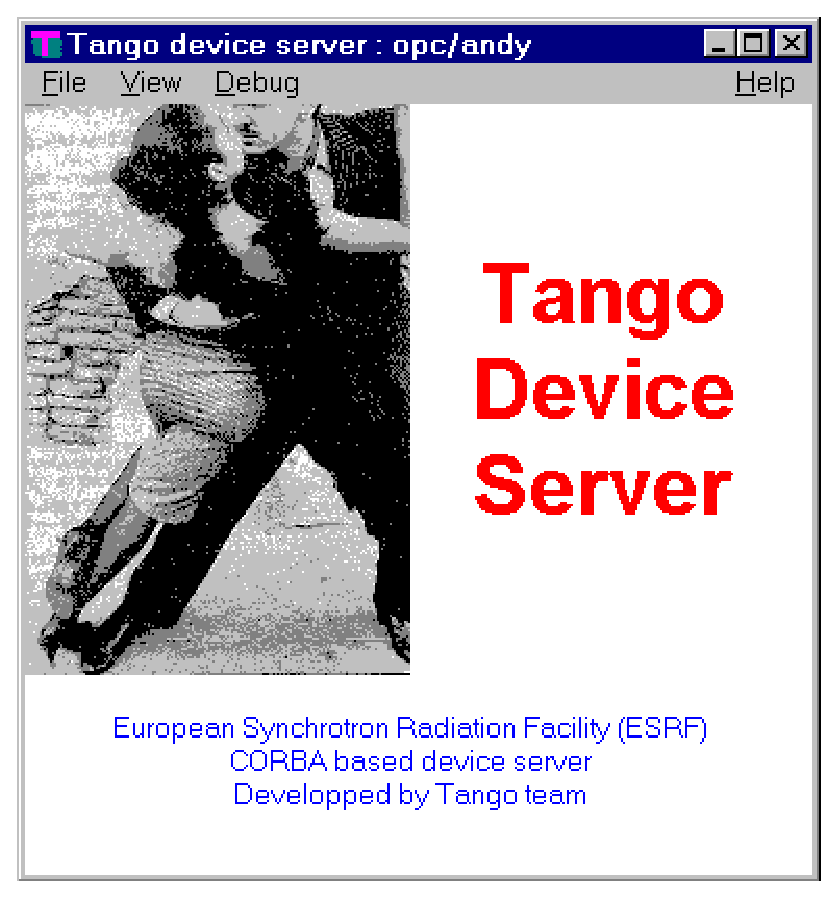
\includegraphics[width=10cm]{ds_writing/nt_server/main}
\end{figure}

\par\end{center}

\vspace{0.3cm}


Four menus are available in this window. The File menu allows the
user to exit the device server. The View menu allows you to display/hide
the device server console window. The Debug menu allows the user to
change the server output verbose\index{verbose} level. All the outputs
goes to the console window even if it is hidden. The Help menu displays
the help window. The device server name is displayed in the window
title. The text displayed at the bottom of the window has a default
value (the one displayed in this window dump) but may be changed by
the device server programmer using the \emph{set\_main\_window\_text(\index{set-main-window-text})}
method of the Tango::Util class. If used, this method must be called
prior to the call of the \emph{server\_init()\index{server-init}}
method. Refer to \cite{TANGO_ref_man} for a complete description
of this method.


\subsubsection{The console window}

This window looks like :

\vspace{0.3cm}


\begin{center}
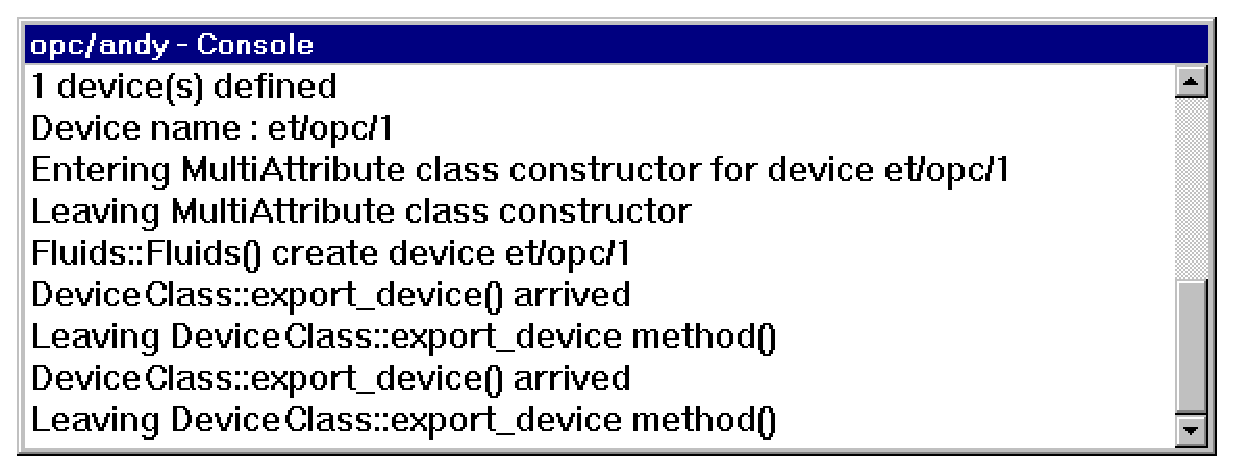
\includegraphics[width=14cm]{ds_writing/nt_server/cons}
\par\end{center}

\vspace{0.3cm}


It simply displays all the logging\emph{\index{logging}} message
when a console target is used in the device server. 


\subsubsection{The help window}

This window looks like :

\vspace{0.3cm}


\begin{center}
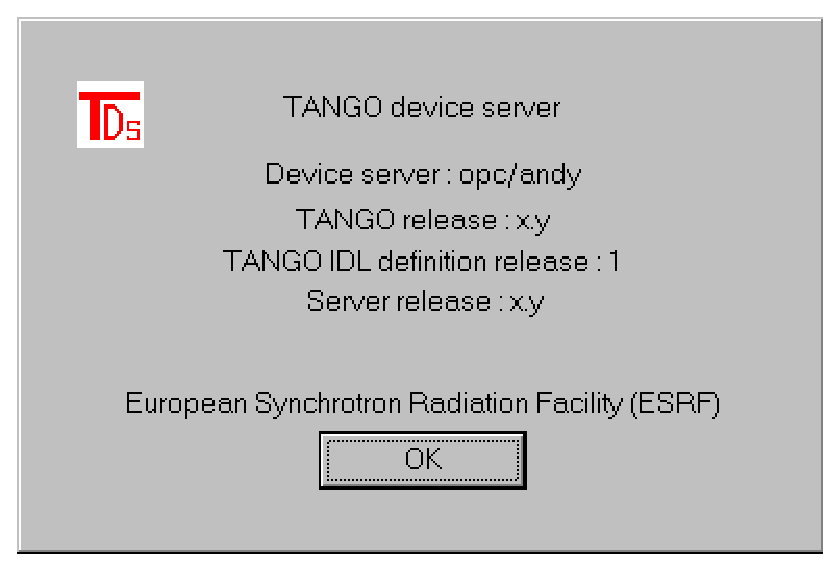
\includegraphics[width=9cm]{ds_writing/nt_server/help}
\par\end{center}



\vspace{0.3cm}


This window displays 
\begin{itemize}
\item The device server name
\item The Tango library release
\item The Tango IDL definition release
\item The device server release. The device server programmer may set this
release number using the \emph{set\_server\_version()\index{set-server-version}}
method of the Tango::Util\index{Util} class. If used, this must be
done prior to the call of the \emph{server\_init()} method. If the
\emph{set\_server\_version()} method is not used, x.y is displays
as version number. Refer to \cite{TANGO_ref_man} for a complete description
of this method.
\end{itemize}

\subsection{MFC device server}

There is no \emph{main} function within a classical MFC\index{MFC}
program. Most of the time, your application is represented by one
instance of a C++ class which inherits from the MFC CWinApp class.
This CWinApp class has several methods that you may overload in your
application class. For a device server to run correctly, you must
overload two methods of the CWinApp class. These methods are the \emph{InitInstance()\index{InitInstance}}
and \emph{ExitInstance()\index{ExitInstance}} methods. The rule of
these methods is obvious following their names.

\textbf{Remember that if the Tango device server graphical user interface
is used, you must link your device server with the Tango windows resource\index{resource}
file}. This is done by adding the Tango resource file to the Project
Settings/Link/Input/Object, library modules window in VC++.


\subsubsection{The InitInstance method}

The code to be added here is the equivalent of the code written in
a classical \emph{main()} function. Don't forget to add the \emph{tango.h}
file in the list of included files.


\begin{minted}[linenos]{cpp}
     1 BOOL FluidsApp::InitInstance()
     2 {
     3    AfxEnableControlContainer();
     4  
     5 // Standard initialization
     6 // If you are not using these features and wish to reduce the size
     7 //  of your final executable, you should remove from the following
     8 //  the specific initialization routines you do not need.
     9  
    10  #ifdef _AFXDLL
    11    Enable3dControls();          // Call this when using MFC in a shared DLL
    12  #else
    13    Enable3dControlsStatic();    // Call this when linking to MFC statically
    14  #endif
    15    Tango::Util *tg;
    16    try
    17    {
    18          
    19        tg = Tango::Util::init(m_hInstance,m_nCmdShow);
    20  
    21        tg->server_init(true);
    22  
    23        tg->server_run();
    24  
    25    }
    26    catch (bad_alloc)
    27    {
    28        MessageBox((HWND)NULL,"Memory error","Command line",MB_ICONSTOP);
    29        return(FALSE);
    30    }
    31    catch (Tango::DevFailed &e)
    32    {
    33        MessageBox((HWND)NULL,,e.errors[0].desc.in(),"Command line",MB_ICONSTOP);
    34        return(FALSE);
    35    }
    36    catch (CORBA::Exception &)
    37    {
    38        MessageBox((HWND)NULL,"Exception CORBA","Command line",MB_ICONSTOP);
    39        return(FALSE);
    40    }
    41  
    42    m_pMainWnd = new CWnd;
    43    m_pMainWnd->Attach(tg->get_ds_main_window());
    44  
    45    return TRUE;
    46  }
\end{minted}


Line 19 : Initialise Tango system. This method also analises the argument
used in command line.

Line 21 : Create Tango classes requesting the Tango Windows graphical\index{graphical}
interface to be used

Line 23 : Start Network listener. Note that under NT, this call returns
in the contrary of UNIX like operating system.

Line 26-30 : Display a message box in case of memory allocation error
and leave method with a return value set to false in order to stop
the process

Line 31-35 : Display a message box in case of error during server
initialization phase.

Line 36-40 : Display a message box in case of error other than memory
allocation. Leave method with a return value set to false in order
to stop the process.

Line 37-38 : Create a MFC\index{MFC} main window and attach the Tango
graphical interface main window to this MFC window.


\subsubsection{The ExitInstance\index{ExitInstance} method}

This method is called when the application is stopped. For Tango device
server, its rule is to destroy the Tango::Util singleton if this one
has been correctly constructed.


\begin{minted}[linenos]{cpp}
     1  int FluidsApp::ExitInstance()
     2  {
     3     bool del = true;
     4  
     5     try
     6     {
     7         Tango::Util *tg = Tango::Util::instance();
     8     }
     9     catch(Tango::DevFailed)
    10     {
    11         del = false;
    12     }
    13  
    14     if (del == true)
    15         delete (Tango::Util::instance());
    16  
    17     return CWinApp::ExitInstance();
    18  }
\end{minted}


Line 7 : Try to retrieve the Tango::Util singleton. If this one has
not been constructed correctly, this call will throw an exception.

Line 9-12 : Catch the exception in case of incomplete Tango::Util
singleton construction

Line 14-15 : Delete the Tango::Util singleton. This will unregister
the Tango device server from the Tango database.

Line 17 : Execute the \emph{ExitInstance} method of the CWinApp class.

If you don't want to use the Tango device server graphical interface,
do not pass any parameter to the \emph{server\_init()\index{server-init}}
method and instead of the code display in lines 37 and 38 in the previous
example of the \emph{InitInstance()} method, use your own code to
initialize your own application.


\subsubsection{Example of how to build a Windows device server MFC based}

This sub-chapter gives an example of what it is needed to do to build
a MFC Windows device server. Rather than being a list of actions to
strictly follow, this is some general rules of how using VC++ to build
a Tango device server using MFC.
\begin{enumerate}
\item Create your device server using Pogo. For a class named MyMotor, the
following files will be needed : \emph{class\_factory.cpp}, \emph{MyMotorClass.h},
\emph{MyMotorClass.cpp}, \emph{MyMotor.h} and \emph{MyMotor.cpp.}
\item On a Windows computer running VC++, create a new project of type ``MFC
app Wizard (exe)'' using static MFC\index{MFC} libs. Ask for a dialog
based project without ActiveX controls.
\item Copy the five files generated by Pogo to the Windows computer and
add them to your project
\item Remove the dialog window files (xxxDlg.cpp and xxxDlg.h), the Resource
include file and the resource script file from your project
\item Add \#include <stdafx.h> as first line of the include files list in
\emph{class\_factory.cpp}, \emph{MyMotorClass.cpp} and \emph{MyMotor.cpp}
file. Also add your own directory and the Tango include directory
to the project pre-compiler include directories list.
\item Enable RTTI in your project settings (see chapter \ref{Compiling NT})
\item Change your application class: 

\begin{enumerate}
\item Add the definition of an \emph{ExitInstance} method in the declaration
file. (xxx.h file)
\item Remove the include of the dialog window file in the xxx.cpp file and
add an include of the Tango master include files (tango.h)
\item Replace the \emph{InitInstance}() method as described in previous
sub-chapter. (xx.cpp file)
\item Add an \emph{ExitInstance()} method as described in previous sub-chapter
(xxx.cpp file)
\end{enumerate}
\item Add all the libraries needed to compile a Tango device server (see
chapter \ref{Compiling NT}) and the Tango resource file to the linker
Object/Libraries modules.
\end{enumerate}

\subsection{Win32 application}

Even if it is more natural to use the C++ structure of the MFC class
to write a Tango device server, it is possible to write a device server
as a Win32\index{Win32} application. Instead of having a \emph{main()}
function as the application entry point, the operating system, provides
a \emph{WinMain()} function as the application entry point. Some code
must be added to this \emph{WinMain\index{WinMain}} function in order
to support Tango device server. Don't forget to add the \emph{tango}.\emph{h}
file in the list of included files. If you are using the project files
generated by Pogo, don't forget to change the linker SUBSYSTEM option
to \textquotedbl{}Windows\textquotedbl{} (Under Linker/System in the
project properties window).


\begin{minted}[linenos]{cpp}
     1  int APIENTRY WinMain(HINSTANCE hInstance,
     2                       HINSTANCE hPrevInstance,
     3                       LPSTR     lpCmdLine,
     4                       int       nCmdShow)
     5  {
     6     MSG msg;
     7     Tango::Util *tg;
     8  
     9     try
    10     {
    11         tg = Tango::Util::init(hInstance,nCmdShow);
    12  
    13         string txt;
    14         txt = "Blabla first line\n";
    15         txt = txt + "Blabla second line\n";
    16         txt = txt + "Blabla third line\n";
    17         tg->set_main_window_text(txt);
    18         tg->set_server_version("2.2");
    19  
    20         tg->server_init(true);
    21  
    22         tg->server_run();
    23  
    24     }
    25     catch (bad_alloc)
    26     {
    27         MessageBox((HWND)NULL,"Memory error","Command line",MB_ICONSTOP);
    28         return (FALSE);
    29     }
    30     catch (Tango::DevFailed &e)
    31     {
    32         MessageBox((HWND)NULL,e.errors[0].desc.in(),"Command line",MB_ICONSTOP);
    33         return (FALSE);
    34     }
    35     catch (CORBA::Exception &)
    36     {
    37         MessageBox((HWND)NULL,"Exception CORBA","Command line",MB_ICONSTOP);
    38         return(FALSE);
    39     }
    40  
    41     while (GetMessage(&msg, NULL, 0, 0)) 
    42     {
    43         TranslateMessage(&msg);
    44         DispatchMessage(&msg);
    45     }
    46  
    47     delete tg;
    48  
    49     return msg.wParam;
    50  }
\end{minted}


Line 11 : Create the Tango::Util\index{Util} singleton

Line 13-18 : Set parameters for the graphical interface

Line 20 : Initialize Tango device server requesting the display of
the graphical interface

Line 22 : Run the device server

Line 25-39 : Display a message box for all the kinds of error during
Tango device server initialization phase and exit WinMain\index{WinMain}
function.

Line 41-45 : The Windows message loop

Line 47 : Delete the Tango::Util singleton. This class destructor
unregisters the device server from the Tango database.

\textbf{Remember that if the Tango device server graphical user interface
is used, you must add the Tango windows resource\index{resource}
file} \textbf{to your project}.

If you don't want to use the tango device server graphical user interface,
do not use any parameter in the call of the \emph{server\_init()\index{server-init}}
method and do not link your device server with the Tango Windows resource
file.


\subsection{Device server as service}

With Windows, if you want to have processes which survive to logoff
sequence and/or are automatically started during computer startup
sequence, you have to write them as service\index{service}. It is
possible to write Tango device server as service. You need to
\begin{enumerate}
\item Write a class which inherits from a pre-written Tango class called
NTService. This class must have a \emph{start\index{start}} method. 
\item Write a main function following a predefined skeleton.
\end{enumerate}

\subsubsection{The service class}

It must inherits from the \emph{NTService} class and defines a \emph{start}
method. The NTService\index{NTService} class must be constructed
with one argument which is the device server executable\index{executable}
name. The \emph{start} method has three arguments which are the number
of arguments passed to the method, the argument list and a reference
to an object used to log info in the NT event system. The first two
args must be passed to the Tango::Util::init method and the last one
is used to log error or info messages. The class definition file looks
like


\begin{minted}[linenos]{cpp}
     1  #include <tango.h>
     2  #include <ntservice.h>
     3  
     4  class MYService: public Tango::NTService
     5  {
     6  public:
     7     MYService(char *);
     8  
     9     void start(int,char **,Tango::NTEventLogger *);
    10  };
\end{minted}




Line 1-2 : Some include files

Line 4 : The MYService class inherits from \emph{Tango::NTService}
class

Line 7 : Constructor with one parameter

Line 9 : The \emph{start()\index{start}} method\\


The class source code looks like


\begin{minted}[linenos]{cpp}
     1  #include <myservice.h>
     2  #include <tango.h>
     3  
     4  using namespace std;
     5  
     6  MYService::MYService(char *exec_name):NTService(exec_name)
     7  {
     8  }
     9  
    10  void MYService::start(int argc,char **argv,Tango::NTEventLogger *logger)
    11  {
    12     Tango::Util *tg;
    13     try
    14     {
    15        Tango::Util::_service = true;
    16  
    17        tg = Tango::Util::init(argc,argv);
    18  
    19        tg->server_init();
    20  
    21        tg->server_run();
    22     }
    23     catch (bad_alloc)
    24     {
    25        logger->error("Can't allocate memory to store device object");
    26     }
    27     catch (Tango::DevFailed &e)
    28     {
    29        logger->error(e.errors[0].desc.in());
    30     }
    31     catch (CORBA::Exception &)
    32     {
    33        logger->error("CORBA Exception");
    34     }
    35  }
\end{minted}




Line 6-8 : The MYService class constructor code.

Line 15 : Set to true the \emph{\_service} static variable of the
\emph{Tango::Util} class.

Line 17-21 : Classical Tango device server startup code

Line 23-34 : Exception management. Please, note that within a service.
it is not possible to print data on a console. This method receives
a reference to a logger\index{logger} object. This object sends all
its output to the Windows event\index{event} system. It is used to
send messages when an exception has occurred.


\subsubsection{The main function}

The main function is used to create one instance of the class describing
the service, to check the service option and to run the service. The
code looks like :


\begin{minted}[linenos]{cpp}
     1  #include <tango.h>
     2  #include <MYService.h>
     3  
     4  using namespace std;
     5  
     6  
     7  int main(int argc,char *argv[])
     8  {
     9     MYService service(argv[0]);
    10          
    11     int ret;
    12     if ((ret = service.options(argc,argv)) <= 0)
    13         return ret;
    14          
    15     service.run(argc,argv);
    16          
    17     return 0;
    18  }
\end{minted}


Line 9 : Create one instance of the MYService class with the executable
name as parameter

Line 12 : Check service option with the \emph{options()} method inherited
from the NTService\index{NTService} class.

Line 15 : Run the service. The \emph{run()} method is inherited from
the NTService class. This method will after some NT initialization
sequence execute the user \emph{start()\index{start}} method.


\subsubsection{Service options and messages}

When a Tango device server is written as a Windows service, it supports
several new options. These option are linked to Windows service\index{service}
usage.

Before it can be used, a service must be installed. A name and a title
is associated to each service. For Tango device server used as service,
the service name is build from the executable name followed by the
underscore character and the instance name. For example, a device
server service executable file named ``opc'' and started with ``fluids''
as instance name, will be named ``opc\_fluids''. The title string
is built from the service executable name followed by the sentence
``Tango device server'' and the instance name between parenthesis.
In the previous example, the service title will be ``opc Tango device
server (fluids)''. Once a service is installed, you can configure
it with the ``Services'' application of the control panel. Services
title are displayed by this application and allow the user to select
one specific service. Once a service is selected, it is possible to
start/stop it and to configure its startup type as manual (with the
Services application) or as automatic. When the automatic mode is
chosen, the service starts when the computer is started. In this case,
the service executable code must resides on the computer local disk.

Tango device server logs message in the Windows event\index{event}
system when the service is started or stopped. You can see these messages
with the ``Event Viewer'' application (Start->Programs->Administrative
tools->Event Viewer) and choose the Application events.

The new options are -i, -s, -u, -h and -d.
\begin{itemize}
\item -i : Install the service\index{service}
\item -s : Install the service and choose the automatic startup mode
\item -u : Un-install the service
\item -dbg : Run in console mode to debug service. The service must have
been installed prior to used it. The classical -v device server option
can be used with the -d option.
\end{itemize}
On the command line, all these options must be used after the device
server instance name (``opc fluids -i'' to install the service,
``opc fluids -u'' to un-install the service, ``opc fluids -v -d''
to debug the service)


\subsubsection{Tango device server using MFC as Windows service}

If your Tango device server uses MFC\index{MFC} and must be written
as a Windows NT service, follow these rules :
\begin{itemize}
\item Don't forget to add the \emph{stdafx.h} file as the first file included
in all the source files making the project.
\item Comment out the definition of VC\_EXTRALEAN in the \emph{stdafx.h}
file.
\item Change the pre-processor definitions, replace \_WINDOWS by \_CONSOLE
\item Add the /SUBSYSTEM:CONSOLE option in the linker options window of
the project settings.
\item Add a call to initialize the MFC (\emph{AfxWinInit()}) in the service
main function
\end{itemize}

\begin{minted}[linenos]{cpp}
     1  int main(int argc,char *argv[])
     2  {
     3     if (!AfxWinInit(::GetModuleHandle(NULL),NULL,::GetCommandLine(),0))
     4     {
     5        cerr << "Can't initialise MFC !" << endl;
     6        return -1;
     7     }
     8  
     9     service serv(argv[0]);
    10  
    11     int ret;
    12     if ((ret = serv.options(argc,argv)) <= 0)
    13          return ret;
    14  
    15     serv.run(argc,argv);
    16  
    17     return 0;
    18  }
\end{minted}


Line 3 : The MFC classes are initialized with the \emph{AfxWinInit()}
function call.


\section{Compiling, linking and executing a TANGO device server process}
\label{sec:Compiling,-linking-and}


\subsection{Compiling and linking a C++ device server}


\subsubsection{On UNIX like operating system }


\paragraph{Supported development tools}

The supported compiler for Linux is \textbf{gcc\index{gcc}} release
3.3 and above. Please, note that to debug a Tango device server running
under Linux\index{Linux}, \textbf{gdb\index{gdb}} release 7 and
above is needed in order to correctly handle threads.


\paragraph{Compiling\index{compiling}}

TANGO for C++ uses omniORB (release 4) as underlying CORBA Object
Request Broker \cite{OOC page} and starting with Tango 8, the ZMQ
library. To compile a TANGO device server, your include search path
must be set to :
\begin{itemize}
\item The omniORB include directory
\item The ZMQ\index{ZMQ} include directory
\item The Tango include directory
\item Your development directory
\end{itemize}

\paragraph{Linking\index{linking} }

To build a running device server process, you need to link your code
with several libraries. Nine of them are always the same whatever
the operating system used is. These nine libraries are:
\begin{itemize}
\item The Tango libraries (called \textbf{libtango} and \textbf{liblog4tango})
\item Three omniORB\index{omniORB} package libraries (called \textbf{libomniORB4},
\textbf{libomniDynamic4} and \textbf{libCOS4)}
\item The omniORB threading library (called \textbf{libomnithread})
\item The ZMQ library (callled \textbf{libzmq})
\end{itemize}
On top of that, you need additional libraries depending on the operating
system :
\begin{itemize}
\item For Linux, add the posix thread library (\textbf{libpthread})
\end{itemize}
The following table summarizes the necessary options to compile a
Tango C++ device server. Please, note that starting with Tango 8 and
for gcc release 4.3 and later, some C++11\index{C++11} code has been
used. This requires the compiler option \textquotedbl{}-std=c++0x\textquotedbl{}.
Obviously, the options -I and -L must be updated to reflect your file
system organization. 

\vspace{0.3cm}


\begin{center}
\begin{longtable}{|c|c|m{70mm}|}
\hline 
Operating system & Compiling option & Linking option\tabularnewline
\hline 
\hline 
Linux gcc & -D\_REENTRANT -std=c++0x -I.. & -L.. -ltango -llog4tango -lomniORB4 -lomniDynamic4 -lCOS4 -lomnithread
-lzmq -lpthread\tabularnewline
\hline 
\end{longtable}
\par\end{center}

\vspace{0.3cm}


The following is an example of a Makefile for Linux. Obviously, all
the paths are set to the ESRF file system structure.


\begin{minted}[linenos]{cpp}
1 #
2 # Makefile to generate a Tango server
3 #
4 
5 CC = c++
6 BIN_DIR = ubuntu1104
7 TANGO_HOME = /segfs/tango
8 
9 INCLUDE_DIRS = -I $(TANGO_HOME)/include/$(BIN_DIR) -I .
10
11 
12 LIB_DIRS = -L $(TANGO_HOME)/lib/$(BIN_DIR)
13 
14 
15 CXXFLAGS = -D_REENTRANT -std=c++0x $(INCLUDE_DIRS)
16 LFLAGS = $(LIB_DIRS) -ltango \
17                      -llog4tango \
18                      -lomniORB4 \
19                      -lomniDynamic4 \
20                      -lCOS4 \
21                      -lomnithread \
22                      -lzmq \
23                      -lpthread
24 
25 
26 SVC_OBJS = main.o \
27            ClassFactory.o \
28            SteppermotorClass.o \
29            Steppermotor.o \
30            SteppermotorStateMachine.o
31 
32 
33 .SUFFIXES: .o .cpp
34 .cpp.o:
35     $(CC) $(CXXFLAGS) -c $<
36 
37 
38 all: StepperMotor
39 
40 StepperMotor: $(SVC_OBJS)
41     $(CC) $(SVC_OBJS) -o $(BIN_DIR)/StepperMotor $(LFLAGS)
42 
43 clean:
44     rm -f *.o core
\end{minted}




Line 5-7 : Define Makefile macros

Line 9-10 : Set the include file search path

Line 12 : Set the linker library search path

Line 15 : The compiler option setting

Line 16-23 : The linker option setting

Line 26-30 : All the object files needed to build the executable

Line 33-35 : Define rules to generate object files

Line 38 : Define a ``all'' dependency

Line 40-41 : How to generate the StepperMotor device server executable

Line 43-44 : Define a ``clean'' dependency


\subsubsection{On Windows using Visual Studio}
\label{Compiling NT}

Supported Windows\index{Windows} compiler for Tango is Visual Studio
2008 (VC 9), Visual Studio 2010 (VC10) and Visual Studio 2013 (VC12).
Most problems in building a Windows device server revolve around the
/M compiler switch family. This switch family controls which run-time
library names are embedded in the object files, and consequently which
libraries are used during linking\index{linking}. Attempt to mix
and match compiler settings and libraries can cause link error and
even if successful, may produce undefined run-time behavior.

Selecting the correct /M switch in Visual Studio is done through a
dialog box. To open this dialog box, click on the ``Project'' menu
(once the correct project is selected in the Solution Explorer window)
and select the ``Properties'' option. To change the compiler switch
open the ``C/C++'' tree and select ``Code Generation''. The following
options are supported.
\begin{itemize}
\item Multithreaded = /MT
\item Multithreaded DLL = /MD
\item Debug Multithreaded = /MTd
\item Debug Multithreaded DLL = /MDd
\end{itemize}
Compiling a file with a value of the /M switch family will impose
at link phase the use of libraries also compiled with the same value
of the /M switch family. If you compiled your source code with the
/MT option (Multithreaded), you must link it with libraries also compiled
with the /MT option.

On both 32 or 64 bits computer, omniORB and TANGO relies on the preprocessor
identifier \textbf{WIN32}\index{WIN32} being defined in order to
configure itself. If you build an application using static libraries
(option /MT or /MTd), you must add \textbf{\_WINSTATIC} to the list
of the preprocessor identifiers. If you build an application using
DLL\index{DLL} (option /MD or /MDd), you must add \textbf{LOG4TANGO\_HAS\_DLL}
and \textbf{TANGO\_HAS\_DLL} to the list of preprocessor identifiers.

To build a running device server process, you need to link your code
with several libraries on top of the Windows libraries. These libraries
are:
\begin{itemize}
\item The Tango libraries (called \textbf{tango.lib} and \textbf{log4tango.lib}
or \textbf{tangod.lib} and \textbf{log4tangod.lib} for debug mode)
\item The omniORB\index{omniORB} package libraries (see next table)\\

\end{itemize}
\begin{center}
\begin{longtable}{|c|c|}
\hline 
Compile mode & Libraries\tabularnewline
\hline 
\hline 
Debug Multithreaded & omniORB4d.lib, omniDynamic4d.lib, omnithreadd.lib and COS4d.lib\tabularnewline
\hline 
Multithreaded & omniORB4.lib, omniDynamic4.lib, omnithread.lib and COS4.lib\tabularnewline
\hline 
Debug Multithreaded DLL & omniORB420\_rtd.lib, omniDynamic420\_rtd.lib, omnithread40\_rtd.lib,\tabularnewline
 & and COS420\_rtd.lib\tabularnewline
\hline 
Multithreaded DLL & omniORB420\_rt.lib, omniDynamic420\_rt.lib, omnithread40\_rt.lib\tabularnewline
 & and COS420\_rt.lib\tabularnewline
\hline 
\end{longtable}
\par\end{center}
\begin{itemize}
\item The ZMQ library (\textbf{zmq.lib} or \textbf{zmqd.lib} for debug mode)
\item Windows network libraries (\textbf{mswsock.lib} and \textbf{ws2\_32.lib})
\item Windows graphic library (\textbf{comctl32.lib})
\end{itemize}
To add these libraries in Visual Studio, open the project property
pages dialog box and open the ``Link'' tree. Select ``Input''
and add these library names to the list of library in the ``Additional
Dependencies'' box. 

The ``Win32 Debug'' or ``Win32 Release'' configuration that you
change within the \textquotedbl{}Configuration Manager\textquotedbl{}
window changes the /M switch compiler. For instance, if you select
a ``Win32 Debug'' configuration in a \textquotedbl{}non-DLL\textquotedbl{}
project, use the omniORB4d.lib, omniDynamic4d.lib and omnithreadd.lib
libraries plus the tangod.lib, log4tangod.lib and zmqd.lib libraries.
If you select the ``Win32 Release'' configuration, use the omniORB4.lib,
omniDynamic4.lib and omnithread.lib libraries plus the tango.lib,
log4tango.lib and zmq.lib libraries.

\textbf{WARNING}: In some cases, the Microsoft Visual Studio wizard
used during project creation generates one include file called \emph{Stdafx.h}.
If this file itself includes windows.h file, you have to add the preprocessor
macro \_WIN32\_WINNT\index{-WIN32-WINNT} and set it to 0x0500.


\subsection{Running a C++ device server}
\label{Env variable}

To run a C++ Tango device server, you must set an environment variable.
This environment variable is called \textbf{TANGO\_HOST\index{TANGO-HOST}}
and has a fixed syntax which is \begin{center}TANGO\_HOST=<host>:<port>\end{center}The
host field is the host name where the TANGO database device server
is running. The port field is the port number on which this server
is listening. For instance, a valid syntax is TANGO\_HOST=dumela:10000.
For UNIX like operating system, setting environment variable is possible
with the \emph{export} or \emph{setenv} command depending on the shell
used. For Windows, setting environment variable is possible with the
``Environment'' tab of the ``System'' application in the control
panel.

If you need to start a Tango device server on a pre-defined port\index{port}
(For Tango database device server or device server without database
usage), you must use one of the underlying ORB option \emph{endPoint}
like \begin{center}myserver myinstance\_name -ORBendPoint giop:tcp::<port
number>\end{center}


\section{Advanced programming techniques}

The basic techniques for implementing device server pattern are required
by each device server programmer. In certain situations, it is however
necessary to do things out of the ordinary. This chapter will look
into programming techniques which permit the device server serve more
than simply the network.


\subsection{Receiving signal}

It is \textbf{UNSAFE} to use any CORBA call in a signal handler. It
is also UNSAFE to use some system calls in a signal handler. Tango
device server solved this problem by using threads\index{thread}.
A specific thread is started to handle signals\index{signal}. Therefore,
every Tango device server is automatically a threaded process. This
allows the programmer to write the code which must be executed when
a signal is received as ordinary code. All device server threads masks
all signals except the specific signal thread which is permanently
waiting for signal. If a signal is sent to a device server process,
only the signal thread will receive it because it is the single thread
which does not mask signals.

Nevertheless, signal management is not trivial and some care have
to be taken. The signal management differs from operating system to
operating system. It is not recommended that you install your own
signal routine using any of the signal routines provided by the operating
system calls or library. 


\subsubsection{Using signal}

It is possible for C++ device server to receive signals from drivers
or other processes. The TDSOM supports receiving signal at two levels:
the device level and the class level. Supporting signal at the device
level means that it is possible to specify interest into receiving
signal on a device basis. This feature is supported via three methods
defined in the DeviceImpl\index{DeviceImpl} class. These methods
are called \emph{register\_signal}, \emph{unregister\_signal} and
s\emph{ignal\_handler}.

The \textbf{\emph{register\_signal\index{register-signal}}} method
has one parameter which is the signal number. This method informs
the device server signal system that the device want to be informed
when the signal passed as parameter is received by the process. There
is a special case for Linux as explained in the previous sub-chapter.
It is possible to register a signal to be executed in the a signal
handler context (with all its restrictions). This is done with a second
parameter to this \emph{register\_signal} method. This second parameter
is simply a boolean data. If it is true, the signal\_handler will
be executed in a signal handler context in the device server main
thread. A default value (false) has been defined for this parameter.

The \textbf{\emph{unregister\_signal\index{unregister-signal}}} method
also have an input parameter which is the signal number. This method
removes the device from the list of object which should be warned
when the signal is received by the process.

The \textbf{\emph{signal\_handler\index{signal-handler}}} method
is the method which is triggered when a signal is received if the
corresponding \emph{register\_signal} has been executed. This method
is defined as virtual and can be redefined by the user. It has one
input argument which is the signal number.

The same three methods also exist in the DeviceClass\index{DeviceClass}
class. Their action and their usage are similar to the DeviceImpl
class methods. Installing a signal at the class level does not mean
that all the device belonging to this class will receive the signal.
This only means that the \emph{signal\_handler} method of the DeviceClass
instance will be executed. This is useful if an action has to be executed
once for a class of devices when a signal is received.

The following code is an example with our stepper motor device server
configured via the database to serve three motors. These motors have
the following names : id04/motor/01, id04/motor/02 and id04/motor/03.
The signal SIGALRM (alarm signal) must be propagated only to the motor
number 2 (id04/motor/02)


\begin{minted}[linenos]{cpp}
 1  void StepperMotor::init_device()
 2  {
 3      cout << "StepperMotor::StepperMotor() create motor " << dev_name << endl;
 4  
 5      long i;
 6  
 7      for (i=0; i< AGSM_MAX_MOTORS; i++)
 8      {
 9          axis[i] = 0;
10          position[i] = 0;
11          direction[i] = 0;
12      }
13  
14      if (dev_name == "id04/motor/02")
15          register_signal(SIGALRM);
16  }
17  
18  StepperMotor::~StepperMotor()
19  {
20      unregister_signal(SIGALRM);
21  }
22  
23  void StepperMotor::signal_handler(long signo)
24  {
25      INFO_STREAM << "Inside signal handler for signal " << signo << endl;
26  
27  //  Do what you want here
28  
29  }
\end{minted}


The \emph{init\_device} method is modified.

Line 14-15 : The device name is checked and if it is the correct name,
the device is registered in the list of device wanted to receive the
SIGALARM signal.

The destructor is also modified

Line 20 : Unregister the device from the list of devices which should
receives the SIGALRM signal. Note that unregister a signal for a device
which has not previously registered its interest for this signal does
nothing.

The \emph{signal\_handler} method is redefined

Line 25 : Print signal number

Line 27 : Do what you have to do when the signal SIGALRM is received.

If all devices must be warned when the device server process receives
the signal SIGALRM, removes line 14 in the \emph{init\_device} method.


\subsubsection{Exiting a device server gracefully}

A device server\index{server} has to exit\index{exit} gracefully
by unregistering itself from the database. The necessary action to
gracefully exit are automatically executed on reception of the following
signal\index{signal} :
\begin{itemize}
\item SIGINT, SIGTERM and SIGQUIT for device server running on Linux
\item SIGINT, SIGTERM, SIGABRT and SIGBREAK for device server running on
Windows
\end{itemize}
This does not prevents device server to also register interest at
device or class levels for those signals. The user installed \emph{signal\_handler\index{signal-handler}}
method will first be called before the graceful exit.


\subsection{Inheriting}
\label{Inheriting}

This sub-chapter details how it is possible to inherit\index{inherit}
from an existing device pattern implementation. As the device pattern
includes more than a single class, inheriting from an existing device
pattern needs some explanations.

Let us suppose that the existing device pattern implementation is
for devices of class A. This means that classes A and AClass already
exists plus classes for all commands offered by device of class A.
One new device pattern\index{pattern} implementation for device of
class B must be written with all the features offered by class A plus
some new one. This is easily done with the inheritance. Writing a
device pattern implementation for device of class B which inherits
from device of class A means :
\begin{itemize}
\item Write the BClass class
\item Write the B class
\item Write B class specific commands
\item Eventually redefine A class commands
\end{itemize}
The miscellaneous code fragments given below detail only what has
to be updated to support device pattern inheritance


\subsubsection{Writing the BClass}

As you can guess, BClass has to inherit from AClass. The \emph{command\_factory\index{command-factory}}
method must also be adapted.


\begin{minted}[linenos]{cpp}
     1  namespace B
     2  {
     3  
     4  class BClass : public A::AClass
     5  {
     6  .....
     7  }
     8  
     9  BClass::command_factory()
    10  {
    11      A::AClass::command_factory();
    12  
    13      command_list.push_back(....);
    14  }
    15  
    16  } /* End of B namespace */
\end{minted}


Line 1 : Open the B namespace

Line 4 : BClass inherits from AClass which is defined in the A namespace.

Line 11 : Only the \emph{command\_factory} method of the BClass will
be called at start-up. To create the AClass commands, the \emph{command\_factory}
method of the AClass must also be executed. This is the reason of
the line

Line 13 : Create BClass commands


\subsubsection{Writing the B class}

As you can guess, B has to inherits\index{inherit} from A.


\begin{minted}[linenos]{cpp}
     1  namespace B
     2  {
     3  
     4  class B : public A:A
     5  {
     6     .....
     7  };
     8  
     9  B::B(Tango::DeviceClass *cl,const char *s):A::A(cl,s)
    10  {
    11     ....
    12     init_device();
    13  }
    14  
    15  void B::init_device()
    16  {
    17     ....
    18  }
    19  
    20  } /* End of B namespace */
\end{minted}


Line 1 : Open the B namespace.

Line 4 : B inherits from A which is defined in the A namespace

Line 9 : The B constructor calls the right A constructor


\subsubsection{Writing B class specific command}

Noting special here. Write these classes as usual


\subsubsection{Redefining A class command\index{command}}

It is possible to redefine a command which already exist in class
A \textbf{only if the command is created} \textbf{using the inheritance\index{inheritance}
model} (but keeping its input and output argument types). The method
which really execute the class A command is a method implemented in
the A class. This method must be defined as \textbf{virtual.} In class
B, you can redefine the method executing the command and implement
it following the needs of the B class.




\subsection{Using another device pattern implementation within the same server}

It is often necessary that inside the same device server\index{server},
a method executing a command needs a command of another class to be
executed. For instance, a device pattern implementation for a device
driven by a serial line class can use the command offered by a serial
line class embedded within the same device server process. To execute
one of the command (or any other CORBA\index{CORBA} operations/attributes)
of the serial line class, just call it as a normal client will do
by using one instance of the DeviceProxy class\emph{.} The ORB will
recognize that all the devices are inside the same process and will
execute calls as a local\index{local} calls. To create the DeviceProxy
class instance, the only thing you need to know is the name of the
device you gave to the serial line device. Retrieving this could be
easily done by a Tango device property. The DeviceProxy class is fully
described in Tango Application Programming Interface (API) reference
WEB pages


\subsection{Device pipe\index{pipe}}

What a Tango device pipe is has been defined in the Chapter 3 about
device server model. How you read or write a pipe in a client software
is documented in chapter 4 about the Tango API. In this section, we
describe how you can read/write into/from a device pipe on the server
side (In a Tango class with pipe).


\subsubsection{Client reading a pipe}

When a client reads a pipe, the following methods are executed in
the Tango class:
\begin{enumerate}
\item The \emph{always\_executed\_hook()} method.
\item A method called \emph{is\_<pipe\_name>\_allowed()}. The rule of this
method is to allow (or disallow) the next method to be executed. It
is usefull for device with some pipes which can be read only in some
precise conditions. It has one parameter which is the request type
(read or write)
\item A method called \emph{read\_<pipe\_name>()}. The aim of this method
is to store the pipe data in the pipe object. It has one parameter
which is a reference to the Pipe object to be read.
\end{enumerate}
The figure \ref{r_pipe_timing_fig-1} is a drawing of these method
calls sequencing for our class StepperMotor with one pipe named DynData.
\begin{figure}[H]
\begin{centering}
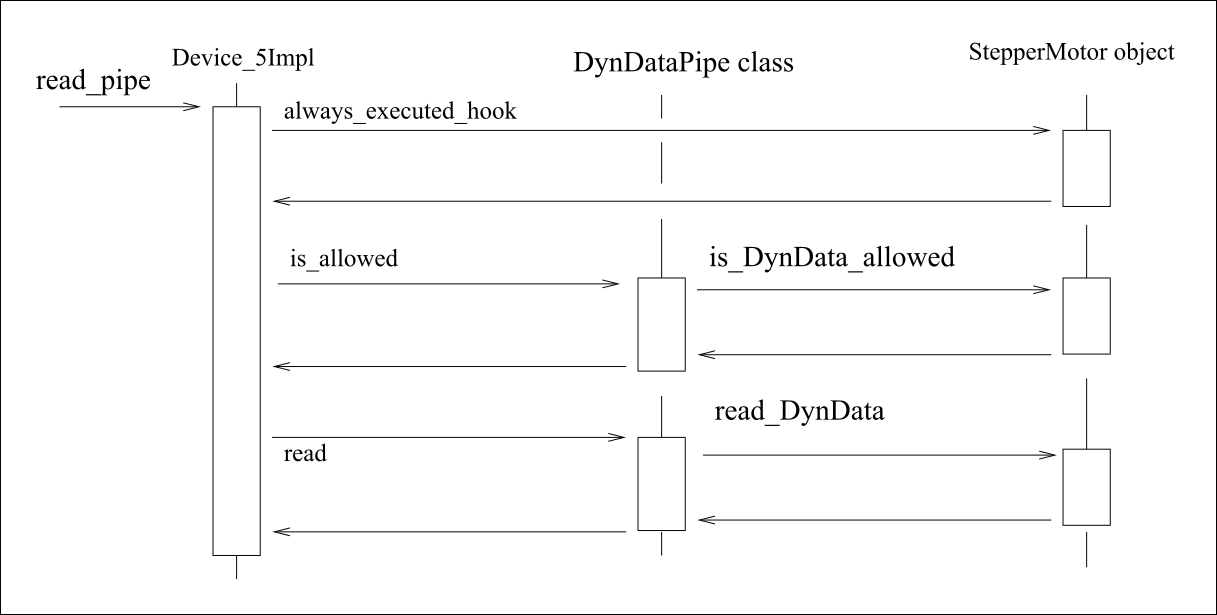
\includegraphics[scale=0.7]{ds_writing/r_pipe}
\par\end{centering}

\protect\caption{Read pipe sequencing}
\label{r_pipe_timing_fig-1}
\end{figure}


The class DynDataPipe is a simple class which follow the same skeleton
from one Tango class to another. Therefore, this class is generated
by the Tango code generator Pogo and the Tango class developper does
not have to modify it. The method \emph{is\_DynData\_allowed()} is
relatively simple and in most cases the default code generated by
Pogo is enough. The method \emph{read\_DynData()} is the method on
which the Tango class developper has to concentrate on. The following
code is one example of these two methods.


\begin{minted}[linenos]{cpp}
     1  bool StepperMotor::is_DynData_allowed(Tango::PipeReqType req)
     2  {
     3      if (get_state() == Tango::ON)
     4          return true;
     5      else
     6          return false;
     7  }
     8
     9  void StepperMotor::read_DynData(Tango::Pipe &pipe)
    10  {
    11      nb_call++;
    12      if (nb_call % 2 == 0)
    13      {
    14          pipe.set_root_blob_name("BlobCaseEven");
    15
    16          vector<string> de_names {"EvenFirstDE","EvenSecondDE"};
    17          pipe.set_data_elt_names(de_names);
    18
    19          dl = 666;
    20          v_db.clear();
    21          v_db.push_back(1.11);
    22          v_db.push_back(2.22);
    23
    24          pipe << dl << v_db;
    25      }
    26      else
    27      {
    28          pipe.set_root_blob_name("BlobCaseOdd");
    29
    30          vector<string> de_names {"OddFirstDE"};
    31          pipe.set_data_elt_names(de_names);
    32
    33          v_str.clear();
    34          v_str.push_back("Hola");
    35          v_str.push_back("Salut");
    36          v_str.push_back("Hi");
    37
    38          pipe << v_str;
    39      }
    40  }
\end{minted}


The \emph{is\_DynData\_allowed} method is defined between lines 1
and 7. It is allowed to read or write the pipe only is the device
state is ON. Note that the input parameter req is not used. The parameter
allows the user to know the type of request. The data type PipeReqType
is one enumeration with two possible values which are READ\_REQ and
WRITE\_REQ.

The \emph{read\_DynData} method is defined between lines 9 and 40.
If the number of times this method has been called is even, the pipe
contains two data elements. The first one is named EvenFirstDE and
its data is a long. The second one is named EvenSecondDE and its data
is an array of double. If the number of call is odd, the pipe contains
only one data element. Its name is OddFirstDe and its data is an array
of strings. Data are inserted into the pipe at lines 24 and 38. The
variables nb\_call, dl, v\_db and v\_str are device data member and
therefore declare in the .h file. Refer to pipe section in chapter
3 and to the API reference documentation (in Tango WEB pages) to learn
more on how you can insert data into a pipe and to know how data are
organized within a pipe.


\subsubsection{Client writing a pipe}

When a client writes a pipe, the following methods are executed in
the Tango class:
\begin{enumerate}
\item The \emph{always\_executed\_hook()} method.
\item A method called \emph{is\_<pipe\_name>\_allowed()}. The rule of this
method is to allow (or disallow) the next method to be executed. It
is usefull for device with some pipes which can be read only in some
precise conditions. It has one parameter which is the request type
(read or write)
\item A method called \emph{write\_<pipe\_name>()}. It has one parameter
which is a reference to the WPipe object to be written. The aim of
this method is to get the data to be written from the WPipe oject
and to write them into the corresponding Tango class objects.
\end{enumerate}
The figure \ref{w_pipe_timing_fig-1-1} is a drawing of these method
calls sequencing for our class StepperMotor with one pipe named DynData.
\begin{figure}[H]
\begin{centering}
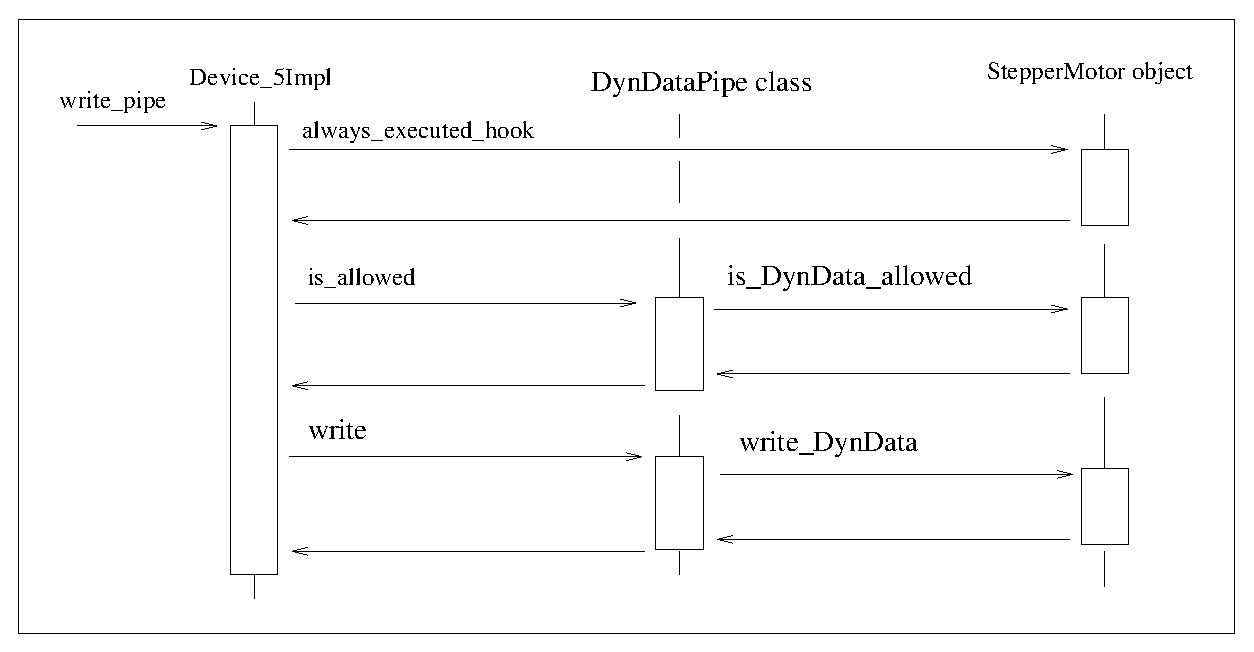
\includegraphics[scale=0.7]{ds_writing/w_pipe}
\par\end{centering}

\protect\caption{Write pipe sequencing}
\label{w_pipe_timing_fig-1-1}
\end{figure}


The class DynDataPipe is a simple class which follow the same skeleton
from one Tango class to another. Therefore, this class is generated
by the Tango code generator Pogo and the Tango class developper does
not have to modify it. The method \emph{is\_DynData\_allowed()} is
relatively simple and in most cases the default code generated by
Pogo is enough. The method \emph{write\_DynData()} is the method on
which the Tango class developper has to concentrate on. The following
code is one example of the \emph{write\_DynData()} method.


\begin{minted}[linenos]{cpp}
     1  void StepperMotor::write_DynData(Tango::WPipe &w_pipe)
     2  {
     3     string str;
     4     vector<float> v_fl;
     5
     6     w_pipe >> str >> v_fl;
     7     .....
     8  }
\end{minted}


In this example, we know that the pipe will always contain a srting
followed by one array of float. On top of that, we are not niterested
by the

data element names. Data are extracted from the pipe at line 6 and
are available for further use starting at line 7. If the content of
the pipe is not a string followed by one array of float, the data
extraction line (6) will throw one exception which will be reported
to the client who has tried to write the pipe. Refer to pipe section
in chapter 3 and to the API reference documentation (in Tango WEB
pages) to learn more on how you can insert data into a pipe and to
know how data are organized within a pipe.

\bigskip{}


\begin{center}

\label{BlackPicture}\includegraphics[scale=0.6]{dance/tango-08-39}

\end{center}
